
\chapter{Derivaci\'{o}n}

\section{Definici\'{o}n de derivada}

Sea $f$ una funci\'{o}n definida en el punto $c\in\left]  a,b\right[  $. Se
define la derivada%
\index{Derivada!Definici\'{o}n de --|textbf}
de $f$ en $x=c$ como%
\begin{equation}
f^{\prime}\left(  c\right)  :=\lim_{h\rightarrow0}\frac{f\left(  c+h\right)
-f\left(  c\right)  }{h} \label{d1}%
\end{equation}
si dicho l\'{\i}mite existe.

Precisando esta idea, ya que%
\[%
\begin{tabular}
[c]{lll}%
$\dfrac{f(c+h)-f(c)}{h}\rightarrow f^{\prime}(c)$ & , cuando & $h\rightarrow
0,$%
\end{tabular}
\]
se tiene que para todo $r>0$, existe $\delta>0$ tal que
\[
\left\vert \frac{f(c+h)-f(c)}{h}-f^{\prime}(c)\right\vert <r,\text{ si
}|h|<\delta.
\]
Para un tal $h$ escribamos
\begin{equation}
E_{c}(h):=f(c+h)-f(c)-hf^{\prime}(c). \label{funcerror}%
\end{equation}
De (\ref{funcerror}) se tiene que%
\begin{equation}
f(c+h)=f(c)+hf^{\prime}(c)+E_{c}(h), \label{diferencial}%
\end{equation}
y como
\begin{align*}
\lim_{h\rightarrow0}\frac{E_{c}(h)}{h}  &  =\lim_{h\rightarrow0}%
\frac{f(c+h)-f(c)}{h}-f^{\prime}(c)\\
&  =0,
\end{align*}
se pone de presente que $f(c+h)\approx f(c)+hf^{\prime}(c),$ si $h\approx0$;
por lo cual se acostumbra describir a $E_{c}$ como una funci\'{o}n
\index{Funci\'{o}n!-- de error}%
de error en la aproximaci\'{o}n de $f(c+h)$ por $f(c)+hf^{\prime}(c)$. La
funci\'{o}n lineal
\begin{figure}
\centering
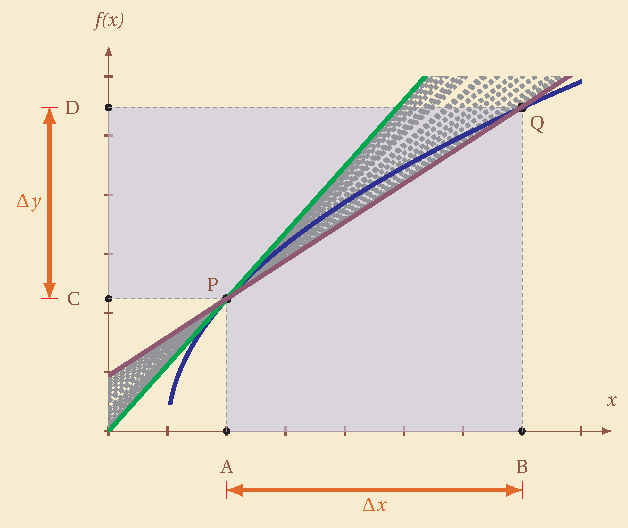
\includegraphics[scale=0.8]{derivada-sec-4.pdf} 
\caption{\protect Aproximaci\'on lineal de $f$ en $c$}
\end{figure}
\begin{equation}
g(x)=f(c)+(x-c)f^{\prime}(c) \label{aproxlinfvsc}%
\end{equation}
(cuya gr\'{a}fica es la ecuaci\'{o}n de la recta tangente en $(c,f(c))$. Ver
figura \ref{difeecni}) es entonces una aproximaci\'{o}n de $f$ en las
vecindades de $c$.
El incremento de $f$ es dado por la
\index{Aplicaci\'{o}n lineal|textbf}%
aplicaci\'{o}n lineal
\begin{equation}
h\longmapsto f^{\prime}(c)h, \label{defdif}%
\end{equation}
la cual es usualmente denominada la \textbf{diferencial%
\index{Diferencial|textbf}%
} de $f$ en $c$.
La existencia de una aplicaci\'{o}n lineal y de una funci\'{o}n de error como
en (\ref{diferencial}) caracteriza a funciones denominadas
\textbf{diferenciables}.
\index{Funciones!-- diferenciables}%
El concepto de diferenciabilidad, para funciones reales de variable real,
coincide as\'{\i} con el de derivabilidad. Por lo tanto $f$ con las
condiciones indicadas en la definici\'{o}n de derivada, se denomina
\textbf{diferenciable%
\index{Funci\'{o}n!-- diferenciable}%
} en $c$ si, y s\'{o}lo si existen una aplicaci\'{o}n lineal%
\[
f_{c}^{\prime}:\rz\longrightarrow\rz,
\]
y una funci\'{o}n
\[
E_{c}:\rz\longrightarrow\rz,
\]
tales que
\begin{align}
f(c+h)  &  =f(c)+f_{c}^{\prime}(h)+E_{c}(h),\label{diferenciabilidadc}\\
\lim_{h\rightarrow0}\frac{E_{c}(h)}{h}  &  =0. \label{errordif}%
\end{align}
La ecuaci\'{o}n (\ref{diferenciabilidadc}) es denominada
\index{F\'{o}rmula de Taylor|textbf}%
\textbf{f\'{o}rmula de Taylor} de primer orden para $f$ en $c$. La funci\'{o}n
$f_{c}^{\prime}$ es la \textbf{diferencial} de $f$ en $c$ citada en
(\ref{defdif}). De la discusi\'{o}n previa se tiene entonces que toda
funci\'{o}n derivable en $x=c,$ es tambi\'{e}n una funci\'{o}n diferenciable
en $x=c$. Rec\'{\i}procamente, si se cumple (\qquad\ref{diferenciabilidadc}) y
(\ref{errordif}), entonces
\begin{align*}
\lim_{h\rightarrow0}\frac{f(c+h)-f(c)}{h}  &  =\lim_{h\rightarrow0}\frac
{f_{c}^{\prime}(h)+Ec(h)}{h}\\
&  =\lim_{h\rightarrow0}\frac{f_{c}^{\prime}(h.1)+E_{c}(h)}{h}\\
&  =\lim_{h\rightarrow0}\frac{hf_{c}^{\prime}(1)+E_{c}(h)}{h}\\
&  =\lim_{h\rightarrow0}\left(  f_{c}^{\prime}(1)+\frac{E_{c}(h)}{h}\right) \\
&  =f_{c}^{\prime}(1),
\end{align*}
lo cual demuestra que $f$ es derivable en $c$ y que
\[
f^{\prime}(c)=f_{c}^{\prime}(1).
\]
Si escribimos $h=x-c$, la derivada puede escribirse tambi\'{e}n como
\begin{equation}
f^{\prime}(c)=\lim_{x\rightarrow c}\frac{f(x)-f(c)}{x-c}.
\end{equation}
Si suponemos $f$ derivable en $x=c,$ es inmediato que
\begin{align*}
\lim_{x\rightarrow c}f(x)  &  =\lim_{x\rightarrow c}\frac{f(x)-f(c)+f(c)}%
{x-c}(x-c)\\
&  =\lim_{x\rightarrow c}\left(  \frac{f(x)-f(c)}{x-c}(x-c)+f(c)\right) \\
&  =f^{\prime}(c)(0)+f(c)\\
&  =f(c)
\end{align*}
y, por lo tanto se cumple el siguiente resultado
\begin{theorem}
\label{d15}Si $f:\left]  a,b\right[  \rightarrow\rz$ es diferenciable%
\index{Funci\'{o}n!-- continua}
en $x=c\in\left]  a,b\right[  $. Entonces $f$ es continua en $x=c$.
\end{theorem}
Ell rec\'{\i}proco es falso en general, como ejemplo tomemeos la funci\'{o}n
valor absoluto
\[
f(x)=|x|,
\]
la cual es continua en $x=0$, pero no es diferenciable en el mismo. En
efecto:
\begin{align*}
\lim_{h\rightarrow0^{+}}\frac{|h|}{h}  &  =1\\
\lim_{h\rightarrow0^{-}}\frac{|h|}{h}  &  =-1,
\end{align*}
por lo que $f^{\prime}(0)$ no existe.

Si consideramos los valores $x$ para quienes exista el l\'{\i}mite
\begin{equation}
f^{\prime}\left(  x\right)  =\lim_{h\rightarrow0}\frac{f\left(  x+h\right)
-f\left(  x\right)  }{h}. \label{d2}%
\end{equation}
\ Entonces se puede asignar a cada $x$ el n\'{u}mero $f^{\prime}\left(
x\right)  $. De esta manera en $\left(  \ref{d2}\right)  $ se define una nueva
funci\'{o}n llamada la derivada de $f$. Si $f^{\prime}$ es continua decimos
que $f$ es
\index{Funci\'{o}n!-- continuamente diferenciable}%
continuamente diferenciable
\begin{notation}
Si $y=f\left(  x\right)  $, la derivada de $f$ respecto a $x$ puede notarse de
cualquiera de las siguientes maneras%
\[
f^{\prime}\left(  x\right)  \equiv y^{\prime}\equiv\dfrac{dy}{dx}\equiv
\dfrac{d}{dx}f\left(  x\right)  \equiv Df\left(  x\right)  \equiv D_{x}f.
\]
\end{notation}
\begin{definition}
[Derivadas laterales]%
\index{Derivadas!laterales}%
Se define la derivada a la derecha (derivada lateral derecha) de $f$ en $x=c$
como $f_{+}^{\prime}$ donde
\[
f_{+}^{\prime}\left(  c\right)  =\lim_{h\rightarrow0^{+}}\frac{f\left(
c+h\right)  -f\left(  c\right)  }{h}\,\,,
\]
si este l\'{\i}mite existe. An\'{a}logamente, se define la derivada a la
izquierda (derivada lateral izquierda) de $f$ en $x=c$ como $f_{-}^{\prime}$
donde
\[
f_{-}^{\prime}\left(  x_{0}\right)  =\lim_{h\rightarrow0^{+}}\frac{f\left(
c+h\right)  -f\left(  c\right)  }{h}\,\,,
\]
si este l\'{\i}mite existe.\newline De la definici\'{o}n de derivada, se puede
decir que una funci\'{o}n $f$ es derivable en $x=c$ si, y solo si
$f_{+}^{\prime}\left(  c\right)  =f_{-}^{\prime}\left(  c\right)  .$
\end{definition}
\begin{definition}
[Diferenciabilidad en un intervalo]%
\index{Derivabilidad!-- en un intervalo}%
Se dice que $f$ es diferenciable en un intervalo abierto $\left]  a,b\right[
$, si $f$ es diferenciable en cada punto del intervalo $\left]  a,b\right[  .$
\end{definition}
Para intervalos de otro tipo, la exigencia de derivabilidad en los extremos se
puede debilitar, exigiendo simplemente derivabilidad lateral en dichos puntos.
Por ejemplo, diremos que $f:[a,b]\rightarrow\rz$ es diferenciable en el
intervalo cerrado $[a,b]$, si $f$ es diferenciable en el intervalo abierto
$\left]  a,b\right[  ,$ y si adem\'{a}s$\ f_{+}^{\prime}\left(  a\right)  \ $y
$\ f_{-}^{\prime}\left(  b\right)  $ existen.
\subsection{Derivada de orden superior}
Si $f:\left]  a,b\right[  \longrightarrow\rz$ es
\index{Derivadas!-- de orden superior}%
una funci\'{o}n, y si $f$ es diferenciable en $c\in\left]  a,b\right[  $,
entonces el conjunto
\[
U=\{x\in\left]  a,b\right[  \mid f^{\prime}(x)\ \mbox{ \ existe}\}
\]
es no vac\'{\i}o. Definimos
\begin{equation}%
\begin{tabular}
[c]{llll}%
$f^{\prime}:$ & $U$ & $\longrightarrow$ & $\rz$\\
& $x$ & $\longmapsto$ & $f^{\prime}\left(  x\right)  .$%
\end{tabular}
\end{equation}
$f^{\prime}$ es la \textbf{funci\'{o}n derivada%
\index{Funci\'{o}n!-- derivada}%
} de $f$ en $U$.

Por lo tanto, si $f$ es una funci\'{o}n diferenciable en un intervalo, su
derivada $f^{\prime}$ puede tambi\'{e}n ser diferenciable, en tal caso su
derivada se denota por $f^{\prime\prime}$. Es decir, la segunda derivada es la
derivada de la derivada . Y as\'{\i} sucesivamente podr\'{\i}amos continuar
derivando para obtener $f^{\prime\prime\prime}=f^{(3)},$ $f^{\prime
\prime\prime\prime}=f^{(4)},\dots.$\newline En general, se puede denotar las
derivadas de orden superior como%
\[
f^{\left(  n\right)  }\left(  x\right)  =y^{\left(  n\right)  }=\frac{d^{n}%
y}{dx^{n}}=\frac{d}{dx}\left(  \frac{d^{n-1}y}{dx^{n-1}}\right)
\ \ ,si\ \ n\geq2
\]
Tambi\'{e}n es usual escribir $C^{n}\left]  a,b\right[  $ para el conjunto de
todas las funciones con derivadas hasta el orden $n$, al menos, y con dichas
derivadas continuas en el intervalo $\left]  a,b\right[  $, $a,b\in\rz$.%
\index{d@$C^{\infty}\left]  a,b\right[  $}
$C^{\infty}\left]  a,b\right[  $ es el conjunto de todas las funciones con
derivadas continuas de todos los ordenes sobre $\left]  a,b\right[  $.
\subsection{Interpretaci\'{o}n geom\'{e}trica de la
derivada\label{ingeodelader}}
De la discusi\'{o}n previa se tiene que en el caso que $f$ sea derivable en
$x=c,$ existe una aproximaci\'{o}n lineal de $f$ en las vecindades de $c$ dada
por (\ref{aproxlinfvsc}). Lo interesante es que esta ecuaci\'{o}n coincide con
la ecuaci\'{o}n de la recta tangente a la gr\'{a}fica de la funci\'{o}n y la
derivada con la pendiente de dicha recta. Para justificar lo anterior,
consideremos la funci\'{o}n $y=f\left(  x\right)  ,$ con $f$ diferenciable en
$x=c$. Observemos que el cociente $\dfrac{f\left(  c+h\right)  -f\left(
c\right)  }{h}$ representa la pendiente de la recta secante que pasa por los
puntos $\left(  c,f\left(  c\right)  \right)  $ y $\left(  c+h,f\left(
c+h\right)  \right)  $ (ver figura \ref{recsec1} )$.$ Al tomar l\'{\i}mite
cuando $h\rightarrow0$,
\index{Derivada!Interpretaci\'{o}n!geom\'{e}trica|textit}%
la pendiente de la recta secante tiende al valor de la
\index{Recta tangente|textbf}%
pendiente de la recta tangente.\ Por lo tanto $f^{\prime}\left(  c\right)  $
es la pendiente de la recta tangente a la curva $y=f\left(  x\right)  $ en el
punto $\left(  c,f\left(  c\right)  \right)  $ y la ecuaci\'{o}n de la recta
tangente es%
\[
y-f\left(  c\right)  =f^{\prime}\left(  c\right)  \left(  x-c\right)
\]
\begin{figure}[H]
\centering
\includegraphics[scale=0.8]%
{derivada-tan.pdf}%
\caption{Tangente a la gr\'{a}fica de una funci\'{o}n }%
\label{recsec1}%
\end{figure}
Como consecuencia se considera,
\begin{definition}
Sea $f$ una funci\'{o}n derivable en $x=c.$ La recta tangente a la gr\'{a}fica
de $f$ en el punto $\left(  c,f\left(  c\right)  \right)  $ es aquella recta
cuya pendiente est\'{a} dada por $f^{\prime}\left(  c\right)  $.
\end{definition}
Observe que esta definici\'{o}n en ning\'{u}n momento excluye la posibilidad
de que la recta tangente corte a la gr\'{a}fica de la funci\'{o}n en varias
ocasiones .
\subsection{Interpretaci\'{o}n f\'{\i}sica de la derivada}
Consideremos una part\'{\i}cula que se mueve a lo largo de una recta durante
un intervalo de tiempo $t_{0}\leq t\leq t_{1}$, con una ecuaci\'{o}n de
posici\'{o}n dada por $x=x\left(  t\right)  $.%
\index{Derivada!Interpretaci\'{o}n!f\'{\i}sica|textit}%
\index{Funci\'{o}n!-- posici\'{o}n}%
Se conoce como velocidad promedio o velocidad media de la part\'{\i}cula en
$\left[  t_{0},t_{1}\right]  ,$ al cociente%
\[
\frac{\Delta x}{\Delta t}=\frac{x\left(  t_{1}\right)  -x\left(  t_{0}\right)
}{t_{1}-t_{0}}:=\overline{v}.
\]
La velocidad media por lo general no brinda informaci\'{o}n sobre la velocidad
de la part\'{\i}cula en un punto cualesquiera $t_{2}\in\left[  t_{0}%
,t_{1}\right]  .$ Si el movimiento es rectilineo uniforme, es claro que para
todo punto en $\left]  t_{0},t_{1}\right[  $, la%
\index{Velocidad!-- promedio}%
\index{Velocidad!-- instantanea}
velocidad de la part\'{\i}cula estar\'{a} dada por $\overline{v}.$ Pero si el
movimiento no es rectilineo uniforme, el problema debe abordarse de otra forma.
Ahora, como el desplazamiento de la part\'{\i}cula en un intervalo $\left[
t_{2},t_{2}+h\right]  $ viene dado por
\[
\Delta x=x\left(  t_{2}+h\right)  -x\left(  t_{2}\right)  .
\]
Entonces, la velocidad media en dicho intervalo estar\'{a} dada por%
\[
\overline{v}=\frac{x\left(  t_{2}+h\right)  -x\left(  t_{2}\right)  }%
{h}=:\overline{v}_{h}\left(  t_{2}\right)  .
\]
A medida que consideramos $h\approx0,$ es claro que se tendran valores de
velocidades medias para instantes cada vez mas cercanos a $t_{2}.$ Extendiendo
este hecho se define la velocidad instantanea de la part\'{\i}cula en
$t=t_{2}$ al l\'{\i}mite (en caso de existir):
\[
v\left(  t_{2}\right)  =\lim_{h\rightarrow0}\overline{v}_{h}\left(
t_{2}\right)  =\lim_{h\rightarrow0}\frac{x\left(  t_{2}+h\right)  -x\left(
t_{2}\right)  }{h}.
\]
Pero en caso de existir el l\'{\i}mite anterior se tiene que $x^{\prime
}\left(  t_{2}\right)  =\lim\limits_{h\rightarrow0}\dfrac{x\left(
t_{2}+h\right)  -x\left(  t_{2}\right)  }{h}.$ Es decir,%
\[
x^{\prime}\left(  t_{2}\right)  =v\left(  t_{2}\right)  .
\]
Por lo tanto, la derivada de la funci\'{o}n posici\'{o}n en el instante
$t=t_{2}$ representa la velocidad instant\'{a}nea de la part\'{\i}cula en
dicho instante.%
\index{Aceleraci\'{o}n!-- media}%
\index{Aceleraci\'{o}n!-- instantanea}%
En forma an\'{a}loga se muestra que la aceleraci\'{o}n instantanea de la
part\'{\i}cula en el instante $t=t_{2}$ esta dado por%
\[
a\left(  t_{2}\right)  =\lim_{h\rightarrow0}\overline{a}_{h}\left(
t_{2}\right)  =\lim_{h\rightarrow0}\frac{v\left(  t_{2}+h\right)  -v\left(
t_{2}\right)  }{h}.
\]
Por lo cual
\[
a\left(  t_{2}\right)  =v^{\prime}\left(  t_{2}\right)  =x^{\prime\prime
}\left(  t_{2}\right)  .
\]
Si consideramos lo expuesto en \ref{ingeodelader}, es claro que en la
gr\'{a}fica $x\left(  t\right)  $ vs. $t,$ la velocidad en el punto $t_{0}$
viene dada por la pendiente de la recta tangente a la curva en $t_{0}$.
An\'{a}logamente, si tenemos la gr\'{a}fica $v\left(  t\right)  $ vs. $t,$ la
aceleraci\'{o}n en $t_{0}\ $es la pendiente de recta tangente a la curva en
$t_{0}.$%
\begin{center}
\includegraphics[scale=0.6]%
{fig-3-4.pdf}%
\end{center}
\section{Teoremas relativos a la derivada.%
\index{Derivada!Teorema relativos de la --}%
}
En esta secci\'{o}n enunciamos sin demostraci\'{o}n algunos teoremas
importantes para el c\'{a}lculo de derivadas.
\begin{theorem}
\label{d3}Si f y g son funciones diferenciables en $\left]  a,b\right[  $,
entonces las funciones $f+g$ ,$f-g$ , $fg$ y $\dfrac{f}{g}$ (con $g\left(
x\right)  \neq0$ ) tambi\'{e}n son diferenciables en $\left]  a,b\right[  $ y
\begin{enumerate}
\item[a.] si $h\left(  x\right)  =f\left(  x\right)  +g\left(  x\right)  $
entonces $h^{\prime}\left(  x\right)  =f^{\prime}\left(  x\right)  +g^{\prime
}\left(  x\right)  .$
\item[b.] si $h\left(  x\right)  =f\left(  x\right)  -g\left(  x\right)  $
entonces $h^{\prime}\left(  x\right)  =f^{\prime}\left(  x\right)  -g^{\prime
}\left(  x\right)  .$
\item[c.] si $h\left(  x\right)  =f\left(  x\right)  g\left(  x\right)  $
entonces $h^{\prime}\left(  x\right)  =f^{\prime}\left(  x\right)  g\left(
x\right)  +f\left(  x\right)  g^{\prime}\left(  x\right)  .$
\item[d.] si $h\left(  x\right)  =\dfrac{f\left(  x\right)  }{g\left(
x\right)  }$ entonces $h^{\prime}\left(  x\right)  =\dfrac{f^{\prime}\left(
x\right)  g\left(  x\right)  -f\left(  x\right)  g^{\prime}\left(  x\right)
}{[g\left(  x\right)  ]^{2}}.$
\end{enumerate}
\end{theorem}
\begin{theorem}
\label{d4}Si $f\left(  x\right)  =cx^{n},\ \ $donde $c$ es una constante y
$n\in\nz$ . Entonces $f^{\prime}\left(  x\right)  =ncx^{n-1}.$
\end{theorem}
\begin{theorem}
\label{d5}Si $f\left(  x\right)  =cx^{r}$ donde $c$ es una constante y
$r\in\rz$. Entonces $f^{\prime}\left(  x\right)  =rcx^{r-1}.$
\end{theorem}
\begin{theorem}
\label{d6}Si $f\left(  x\right)  =c\ \ \forall x\in\left]  a,b\right[  $,
donde c es una constante. Entonces $f^{\prime}\left(  x\right)  =0.$
\end{theorem}
\begin{theorem}
\label{d376} Si $f\left(  x\right)  =\sum_{k=0}^{k=n}a_{k}x^{k}$es una
funci\'{o}n polinomica, se tiene que
\[
f^{\prime}\left(  x\right)  =\sum_{k=1}^{k=n}ka_{k}x^{k-1}.
\]
\end{theorem}
\begin{theorem}
[Derivada de las funciones trigonometricas]%
\index{Derivada!-- de funciones!trigonom\'{e}tricas|textit}%
\label{d7} \textcolor{white}{.}
\begin{enumerate}
\item[a.] Si $f\left(  x\right)  =\operatorname{sen}x$. Entonces $f^{\prime
}\left(  x\right)  =\cos x$.
\item[b.] Si $f\left(  x\right)  =\cos x$. Entonces $f^{\prime}\left(
x\right)  =-\operatorname{sen}x$.
\item[c.] Si $f\left(  x\right)  =\tan x$. Entonces $f^{\prime}\left(
x\right)  =\sec^{2}x$.
\item[d.] Si $f\left(  x\right)  =\cot x$. Entonces $f^{\prime}\left(
x\right)  =-\csc^{2}x$.
\item[e.] Si $f\left(  x\right)  =\sec x$. Entonces $f^{\prime}\left(
x\right)  =\sec x\tan x$.
\item[f.] Si $f\left(  x\right)  =\csc x$. Entonces $f^{\prime}\left(
x\right)  =-\csc x\cot x$.
\end{enumerate}
\end{theorem}
\begin{theorem}
\label{d8}
\index{Regla de la cadena}%
Supongamos que $g$ es diferenciable en $x$, y $f$ es diferenciable en
$g\left(  x\right)  .$ Entonces la funci\'{o}n $h\left(  x\right)  =f\left(
g\left(  x\right)  \right)  $ es diferenciable en $x$ y
\begin{equation}
h^{\prime}\left(  x\right)  =f^{\prime}\left(  g\left(  x\right)  \right)
\cdot g^{\prime}\left(  x\right)  \label{cadena}%
\end{equation}
\end{theorem}
La ecuaci\'{o}n (\ref{cadena}) es denominada usualmente \textbf{regla de la
cadena} para la derivada de funciones compuestas. Si escribimos
$u=f(g(x)),y=g(x)$, entonces $u=f(y)$ y la ecuaci\'{o}n (\ref{cadena}) adopta
la forma
\begin{equation}
\frac{du}{dx}=\frac{du}{dy}\frac{dy}{dx}. \label{cadena2}%
\end{equation}
\begin{theorem}
[Derivada de la funci\'{o}n exponencial y logar\'{\i}tmica]\label{d9}%
\textcolor{white}{.}\label{d7 copy(1)}
\begin{enumerate}
\item[a.] Si $f\left(  x\right)  =\ln x$.%
\index{Derivada!-- de funciones!trascendentes|textit}
Entonces $f^{\prime}\left(  x\right)  =\dfrac{1}{x}$.
\item[b.] Si $f\left(  x\right)  =\ln\left\vert g\left(  x\right)  \right\vert
$. Entonces $f^{\prime}\left(  x\right)  =\dfrac{g^{\prime}\left(  x\right)
}{g\left(  x\right)  }$.
\item[c.] Si $f\left(  x\right)  =\log_{a}x$. Entonces $f^{\prime}\left(
x\right)  =\dfrac{1}{x\ln a}$.
\item[d.] Si $f\left(  x\right)  =e^{x}$. Entonces$\ \ f^{\prime}\left(
x\right)  =e^{x}$.
\item[e.] Si $f\left(  x\right)  =e^{g\left(  x\right)  }$. Entonces
$f^{\prime}\left(  x\right)  =g^{\prime}\left(  x\right)  e^{g\left(
x\right)  }$.
\item[f.] Si $f\left(  x\right)  =a^{x}$ $\left(  a>0,\ a\neq1\right)  $.
Entonces $f^{\prime}\left(  x\right)  =a^{x}\ln a$.
\end{enumerate}
\end{theorem}
\begin{theorem}
[Derivada de la funciones trigonometricas inversas]\label{d10}
\textcolor{white}{.}%
\index{Derivada!-- de funciones!trigonom\'{e}tricas inversas|textit}%
\begin{enumerate}
\item[a.] Si $f\left(  x\right)  =\arcsin x,\left\vert x\right\vert <1$.
Entonces $f^{\prime}\left(  x\right)  =\dfrac{1}{\sqrt{1-x^{2}}}$.
\item[b.] Si $f\left(  x\right)  =\arccos x,\left\vert x\right\vert <1$.
Entonces $f^{\prime}\left(  x\right)  =\dfrac{-1}{\sqrt{1-x^{2}}}$.
\item[c.] Si $f\left(  x\right)  =\arctan x,x\in\left]  -\infty,+\infty
\right[  $. Entonces $f^{\prime}\left(  x\right)  =\dfrac{1}{1+x^{2}}$.
\item[d.] Si $f\left(  x\right)  =\operatorname*{arccot}x,x\in\left]
-\infty,+\infty\right[  $. Entonces $f^{\prime}\left(  x\right)  =-\dfrac
{1}{1+x^{2}}.$
\item[e.] Si $f\left(  x\right)  =\operatorname*{arcsec}x,\left\vert
x\right\vert >1$. Entonces $f^{\prime}\left(  x\right)  =\dfrac{1}{\left\vert
x\right\vert \sqrt{x^{2}-1}}.$
\item Si $f\left(  x\right)  =\operatorname*{arccsc}x,\left\vert x\right\vert
>1.$ Entonces $f^{\prime}\left(  x\right)  =-\dfrac{1}{\left\vert x\right\vert
\sqrt{x^{2}-1}}.$
\end{enumerate}
\end{theorem}
\begin{theorem}
[Regla de L'H\^{o}pital]%
\index{e@Regla de L'H\^{o}pital}%
\label{d11} \textcolor{white}{.} Si f y g son funciones continuamente
diferenciables en el intervalo $I=\left]  a-\delta,a+\delta\right[  ,\delta
>0$, y supongamos que $f\left(  a\right)  =0$, $g\left(  a\right)  =0$ y
$g^{\prime}\left(  x\right)  \neq0$ para $x\neq a\ $. Entonces
\[
\lim\limits_{x\rightarrow a}\dfrac{f\left(  x\right)  }{g\left(  x\right)
}=\lim\limits_{x\rightarrow a}\dfrac{f^{\prime}\left(  x\right)  }{g^{\prime
}\left(  x\right)  }.
\]
\end{theorem}
\section{Derivaci\'{o}n impl\'{\i}cita%
\index{Derivada!-- impl\'{\i}cita}%
}
Si una ecuaci\'{o}n en dos variables define impl\'{\i}citamente una variable
como funci\'{o}n diferenciable de la otra, podemos entonces utilizar la regla
de la cadena para encontrar la derivada de dicha funci\'{o}n. Para ser m\'{a}s
precisos supongamos
\begin{itemize}
\item $F(x,y)=0$ es una ecuaci\'{o}n en las variables $x$ y $y.$
\item $y=f(x)$ est\'{a} definida impl\'{\i}citamente por $F(x,y)=0$, y
\item $f$ es diferenciable en alg\'{u}n abierto $\left]  a,b\right[  $.
\end{itemize}
De los tres items anteriores, tenemos la ecuaci\'{o}n
\index{Funci\'{o}n!-- definida implicitamente}
\[
g(x)=F(x,f(x))=0,
\]
de donde se tiene que $g^{\prime}(x)=0$. Es decir, podemos diferenciar en
ambos miembros y obtener as\'{\i} una ecuaci\'{o}n \textquotedblleft
diferencial\textquotedblright\
\[
\frac{d}{dx}(F(x,y))=G(x,y,y^{\prime})=0
\]
la cual es satisfecha por $f$ y su derivada $f^{\prime}$.
Consideremos, por ejemplo, la ecuaci\'{o}n
\[
x^{2}+y^{2}=1
\]
la cual es la ecuaci\'{o}n de la circunferencia unitaria centrada en $\left(
0,0\right)  $ y, por lo tanto su conjunto soluci\'{o}n no es una funci\'{o}n.
Sin embargo, las ecuaciones:
\begin{align}
y=f(x)  &  =\sqrt{1-x^{2}},\label{unafuncion}\\
y=g(x)  &  =-\sqrt{1-x^{2}} \label{dosfuncion}%
\end{align}
definen funciones impl\'{\i}citas en la ecuaci\'{o}n de la circunferencia.
Para $x\in\left]  -1,1\right[  $, se tiene
\begin{align*}
y^{\prime}=f^{\prime}(x)  &  =-\frac{x}{\sqrt{1-x^{2}}}\\
&  =-\frac{x}{y}\\
y^{\prime}=g^{\prime}(x)  &  =\frac{x}{\sqrt{1-x^{2}}}\\
&  =-\frac{x}{y}%
\end{align*}
N\'{o}tese as\'{\i} que , en ambos casos se satisface la ecuaci\'{o}n
diferencial
\[
y^{\prime}=-\frac{x}{y}.
\]
Esta \'{u}ltima ecuaci\'{o}n se pudo obtener por derivaci\'{o}n
impl\'{\i}cita; es decir, directamente de la ecuaci\'{o}n de la
circunferencia, derivando, respecto a $x$, t\'{e}rmino a t\'{e}rmino y miembro
a miembro en dicha ecuaci\'{o}n, como se muestra a continuaci\'{o}n,
\begin{align*}
\frac{d}{dx}(x^{2}+y^{2})  &  =\frac{d}{dx}(1)\\
2x+2yy^{\prime}  &  =0\\
y^{\prime}  &  =-\frac{x}{y}.
\end{align*}
\subsection{Derivada de la funci\'{o}n inversa%
\index{Derivada!-- de funciones!inversas|textit}%
}
Si $f:\left]  a,b\right[  \in\rz$ es una funci\'{o}n invertible y
diferenciable, con inversa $f^{-1}:\operatorname*{Ran}(f)\longrightarrow
\left]  a,b\right[  $, entonces
\[
f\circ f^{-1}=Id_{\operatorname*{Ran}(f)}%
\]
es diferenciable. Si $f^{-1}$ es diferenciable \footnote{Puede demostrarse que
funciones con derivada no nula en un punto son uno-a-uno en alguna vecindad de
dicho punto y que la inversa es diferenciable en la im\'{a}gen de dicho
punto.} la regla de la cadena produce
\begin{align*}
(f\circ f^{-1})^{\prime}(x)  &  =1\\
f^{\prime}(f^{-1}(x))(f^{-1})^{\prime}(x)  &  =1
\end{align*}
de donde se sigue que
\begin{equation}
(f^{-1})^{\prime}(x)=\frac{1}{f^{\prime}(f^{-1}(x))}
\label{derivadadeinversas}%
\end{equation}
En general, si escribimos $y=f^{-1}(x)$, por definici\'{o}n de inversa se
tiene que
\[
x=f(y).
\]
Derivando con relaci\'{o}n a $x$ y usando la regla de la cadena, tenemos:
\begin{align*}
\frac{d}{dx}(x)  &  =\frac{d}{dx}(f(y))\\
1  &  =f^{\prime}(y)\frac{dy}{dx}\\
\frac{dy}{dx}  &  =\frac{1}{f^{\prime}(y)}\\
&  =\frac{1}{\frac{dx}{dy}}%
\end{align*}
\subsection{Derivaci\'{o}n logar\'{\i}tmica}%
\index{Derivaci\'{o}n!-- logaritmica}%
Si $x\in\rz$, $x\neq0$, entonces $\ln(|x|)$ est\'{a} definido. Si consideramos
la funci\'{o}n
\[
g(x)=\ln(|x|)
\]
con dominio $\rz-\{0\}$, entonces $g$ es una compuesta de funciones
diferenciables en el dominio indicado. Tenemos
\begin{align*}
g^{\prime}(x)  &  =\frac{1}{|x|}\frac{d}{dx}\left(  |x|\right) \\
&  =\frac{1}{|x|}\frac{x}{|x|}\\
&  =\frac{1}{x}%
\end{align*}
Si $r\in\qz$, y $y=x^{r},x>0$, tenemos entonces que
\begin{align*}
\ln(y)  &  =\ln(x^{r})\\
&  =r\ln(x)
\end{align*}
de donde
\begin{align*}
\frac{1}{y}y^{\prime}  &  =r\frac{1}{x}\\
y^{\prime}  &  =ry\frac{1}{x}\\
&  =rx^{r-1}%
\end{align*}
lo que muestra que la regla para la derivada de potencias enteras de $x$ se
extiende a potencias con exponentes racionales. El proceso mostrado en el
c\'{a}lculo de la derivada $y^{\prime}$ es a menudo conocido como
derivaci\'{o}n logar\'{\i}tmica.
\section{Ejercicios resueltos.}
En esta secci\'{o}n se presentan una serie de ejemplo resueltos de c\'{a}lculo
de derivadas de funciones elementales.
\begin{example}
Calcule la derivada de la funci\'{o}n $y=3x^{2}$ utilizando la definici\'{o}n.
\end{example}
\begin{sol}
Tomando $f\left(x\right)=3x^{2}$, es claro que $f\left(x+h\right)
=3(x+h)^{2}$ por lo cual%
\begin{align*}
f^{\prime}(x)=\lim_{h\rightarrow0}\frac{f\left(  x+h\right)  -f\left(
x\right)  }{h}  &  =\lim_{h\rightarrow0}\frac{3\left(  x+h\right)  ^{2}%
-3x^{2}}{h}\\
&  =\lim_{h\rightarrow0}\frac{3x^{2}+6xh+h^{2}-3x^{2}}{h}\\
&  =\lim_{h\rightarrow0}\frac{6xh+h^{2}}{h}=\lim_{h\rightarrow0}\frac{h\left(
6x+h\right)  }{h}\\
&  =\lim_{h\rightarrow0}\left(  6x+h\right)  =6x.
\end{align*}
Entonces, la derivada de $f\left(  x\right)  =3x^{2}$ es $f^{\prime}\left(
x\right)  =6x$.
\end{sol}
\begin{example}
Calcular la derivada de la funci\'{o}n $y=\sqrt{x}$ utilizando la
definici\'{o}n de derivada
\end{example}
\begin{sol}
Como $f\left(x\right)=\sqrt{x}$, se tiene que $f\left(x+h\right)
=\sqrt{x+h}.$ Entonces%
\begin{align*}
f^{\prime}\left(  x\right)   &  =\lim_{h\rightarrow0}\frac{f\left(
x+h\right)  -f\left(  x\right)  }{h}=\lim_{h\rightarrow0}\frac{\sqrt{\left(
x+h\right)  }-\sqrt{x}}{h}\\
&  =\lim_{h\rightarrow0}\frac{\sqrt{\left(  x+h\right)  }-\sqrt{x}}{h}%
\cdot\frac{\sqrt{\left(  x+h\right)  }+\sqrt{x}}{\sqrt{\left(  x+h\right)
}+\sqrt{x}}\\
&  =\lim_{h\rightarrow0}\frac{\left(  x+h\right)  -x}{h\left(  \sqrt{\left(
x+h\right)  }+\sqrt{x}\right)  }=\lim_{h\rightarrow0}\frac{h}{h\left(
\sqrt{\left(  x+h\right)  }+\sqrt{x}\right)  }\\
&  =\lim_{h\rightarrow0}\frac{1}{\sqrt{\left(  x+h\right)  }+\sqrt{x}}%
=\frac{1}{2\sqrt{x}}.
\end{align*}
Por lo tanto, la derivada de $f\left(  x\right)  =\sqrt{x}$ esta dada por
$f^{\prime}\left(  x\right)  =\dfrac{1}{2\sqrt{x}}.$
\end{sol}
\begin{example}
Calcular la derivada de la funci\'{o}n $y=\dfrac{1}{x}$ utilizando la
definici\'{o}n de derivada.
\end{example}
\begin{sol}
En forma similar a los problemas anteriores, calculemos $\lim
\limits_{h\rightarrow0}\dfrac{f\left(  x+h\right)  -f\left(  x\right)  }{h}.$%
\begin{align*}
\lim\limits_{h\rightarrow0}\dfrac{f\left(  x+h\right)  -f\left(  x\right)
}{h}  &  =\lim\limits_{h\rightarrow0}\dfrac{\dfrac{1}{x+h}-\dfrac{1}{x}}{h}\\
&  =\lim\limits_{h\rightarrow0}\dfrac{\dfrac{x-\left(  x+h\right)  }{\left(
x+h\right)  x}}{h}=\lim\limits_{h\rightarrow0}\dfrac{-h}{hx\left(  x+h\right)
}\\
&  =\lim\limits_{h\rightarrow0}\frac{-1}{x\left(  x+h\right)  }=\frac
{-1}{x^{2}}.
\end{align*}
Es decir, la derivada de $f\left(  x\right)  =\dfrac{1}{x}$ es $f^{\prime
}\left(  x\right)  =-\dfrac{1}{x^{2}}.$
\end{sol}
\begin{example}
Calcular la derivada de la funci\'{o}n%
\[
f\left(  x\right)  =20x^{4}-5x^{3}+2x^{2}-5.
\]
\end{example}
\begin{sol}
Usando el teorema \ref{d376} se tiene que%
\[
f^{\prime}\left(x\right)  =80x^{3}-15x^{2}+4x
\]
\end{sol}
\begin{example}
Calcular la derivada de la funci\'{o}n
\[
f\left(x\right)  =\left(6x^{2}+5\right)  \left(x^{3}-3x\right)^{9}.
\]
\end{example}
\begin{sol}
Derivando como un producto y aplicando la regla de la cadena para derivar el
segundo factor se tiene que%
\begin{align*}
f^{\prime}\left(  x\right)   &  =(6x^{2}+5)^{\prime}\cdot\left(
x^{3}-3x\right)  ^{9}+(6x^{2}+5)\cdot\left(  \left(  x^{3}-3x\right)
^{9}\right)  ^{\prime}\\
f^{\prime}\left(  x\right)   &  =\left(  12x\right)  \left(  x^{3}-3x\right)
^{9}+\left(  6x^{2}+5\right)  9\left(  x^{3}-3x\right)  ^{8}\underset{\frac
{d}{dx}\left(  x^{3}-3x\right)  }{\underbrace{\left(  3x^{2}-3\right)  }}\\
&  =3x^{8}\left(  58x^{4}-21x^{2}-45\right)  \left(  x^{2}-3\right)  ^{8}.
\end{align*}
\end{sol}
\begin{example}
Calcular la derivada de la funci\'{o}n
\[
f\left(  x\right)  =\frac{6x^{3}+1}{5x^{2}+3x-4}.
\]
\end{example}
\begin{sol}
Ya que la funci\'{o}n es racional, usando los teoremas \ref{d3}, \ref{d4} y
\ref{d6} se tiene que%
\begin{align*}
f^{\prime}\left(  x\right)   &  =\frac{18x^{2}\left(  5x^{2}+3x-4\right)
-\left(  6x^{3}+1\right)  \left(  10x+3\right)  }{\left(  5x^{2}+3x-4\right)
^{2}}\\
&  =\frac{30x^{4}+36x^{3}-72x^{2}-10x-3}{\left(  5x^{2}+3x-4\right)  ^{2}}.
\end{align*}
\end{sol}
\begin{example}
Calcular la derivada de la funci\'{o}n
\[
f\left(  x\right)  =\frac{x\operatorname{sen}x}{\operatorname{sen}x+\cos x}%
\]
\end{example}
\begin{sol}
Los teoremas \ref{d3}, \ref{d4}, \ref{d6} y \ref{d7} implican que%
\begin{align*}
f^{\prime}\left(  x\right)   &  =\frac{\left(  \operatorname{sen}x+x\cos
x\right)  \left(  \operatorname{sen}x+\cos x\right)  -\left(
x\operatorname{sen}x\right)  \left(  \cos x-\operatorname{sen}x\right)
}{\left(  \operatorname{sen}x+\cos x\right)  ^{2}}\\
&  =\frac{\operatorname{sen}x\cos x+1+x-\cos^{2}x}{\left(  \operatorname{sen}%
x+\cos x\right)  ^{2}}.
\end{align*}
\end{sol}
\begin{example}
Sea%
\[
f\left(  x\right)  =\tan\left(  x^{2}\right)  +\cot\left(  2x\right)  +x^{2}%
\]
Hallar $f^{\prime}\left(  1\right)  \ y$ $f^{\prime}\left(  3\right)  .$
\end{example}
\begin{sol}
Calculemos $f^{\prime}\left(  x\right)  .$ Utilizando los teoremas \ref{d3},
\ref{d5}, \ref{d7} y \ref{d8} se tiene que%
\[
f^{\prime}\left(  x\right)  =2x\sec^{2}\left(  x^{2}\right)  -2\csc^{2}\left(
2x\right)  +2x.
\]
Por lo tanto%
\begin{align*}
f^{\prime}\left(  1\right)   &  =2\sec^{2}\left(  1\right)  -2\csc^{2}\left(
2\right)  +2\approx6.432\\
f^{\prime}\left(  3\right)   &  =6\sec^{2}\left(  9\right)  -2\csc^{2}\left(
6\right)  +6\approx-12.389.
\end{align*}
\end{sol}
\begin{example}
Calcular la derivada de la funci\'{o}n
\[
f\left(  x\right)  =\sqrt{x^{2}+5x+1}%
\]
\end{example}
\begin{sol}
Como $f\left(  x\right)  =\left(  x^{2}+5x+1\right)  ^{%
%TCIMACRO{\U{bd}}%
%BeginExpansion
\frac12
%EndExpansion
}$ los teoremas \ref{d3}, \ref{d4}, \ref{d6}, \ref{d8} implican que%
\begin{align*}
f^{\prime}\left(  x\right)   &  =\frac{1}{2}\left(  x^{2}+5x+1\right)  ^{-%
%TCIMACRO{\U{bd}}%
%BeginExpansion
\frac12
%EndExpansion
}\left(  2x+5\right) \\
&  =\frac{2x+5}{2\sqrt{x^{2}+5x+1}}%
\end{align*}
\end{sol}
\begin{example}
Hallar la segunda derivada de la funci\'{o}n%
\[
f\left(  x\right)  =\frac{x^{2}+4x-1}{x^{2}+x-4}%
\]
\end{example}
\begin{sol}
Calculemos $f^{\prime}\left(  x\right)  $ y seguidamente $f^{\prime\prime
}\left(  x\right)  $%
\begin{align*}
f^{\prime}\left(  x\right)   &  =\frac{\left(  2x+4\right)  \left(
x^{2}+x-4\right)  -\left(  x^{2}+4x-1\right)  \left(  2x+1\right)  }{\left(
x^{2}+x-4\right)  ^{2}}\\
&  =\frac{-3\left(  x^{2}+2x+5\right)  }{\left(  x^{2}+x-4\right)  ^{2}}%
\end{align*}
y como $f^{\prime\prime}=\left(  f^{\prime}\right)  ^{\prime}$
\begin{align*}
f^{\prime\prime}\left(  x\right)   &  =\frac{-3\left(  2x+2\right)  \left(
x^{2}+x-4\right)  ^{2}+\left(  3x^{2}+6x+15\right)  2\left(  x^{2}+x-4\right)
\left(  2x+1\right)  }{\left(  x^{2}+x-4\right)  ^{4}}\\
&  =\frac{6\left(  x^{2}+x-4\right)  \left(  x^{3}+3x^{2}+15x+9\right)
}{\left(  x^{2}+x-4\right)  ^{4}}=\frac{6\left(  x^{3}+3x^{2}+15x+9\right)
}{\left(  x^{2}+x-4\right)  ^{3}}%
\end{align*}
\end{sol}
\begin{example}
[Existencia de tangentes verticales.]%
\index{Recta tangente!-- vertical}%
Sea $f\left(  x\right)  =\left(  x-2\right)  ^{\frac{1}{3}}.$ Pruebe que la
funci\'{o}n es continua en $x=2,$ pero no diferenciable en dicho punto.
\end{example}
\begin{sol}
La continuidad de $f$ en $x=2$ es inmediata, debido a que
\[
\lim_{x\rightarrow2^{-}}\left(  x-2\right)  ^{\frac{1}{3}}=\lim_{x\rightarrow
2^{+}}\left(  x-2\right)  ^{\frac{1}{3}}=0=f\left(  2\right)  .
\]
Veamos que $f$ no es derivable en $x=2.$ En efecto, se tiene que
\begin{align*}
f^{\prime}\left(  2\right)   &  =\lim_{x\rightarrow2}\frac{f\left(  x\right)
-f\left(  2\right)  }{x-2}\\
&  =\lim_{x\rightarrow2}\frac{\left(  x-2\right)  ^{\frac{1}{3}}-0}{x-2}%
=\lim_{x\rightarrow2}\frac{1}{\left(  x-2\right)  ^{\frac{2}{3}}}=+\infty.
\end{align*}
Se observa que la gr\'{a}fica de $f\left(  x\right)  =\left(  x-2\right)
^{\frac{1}{3}},$ posee una tangente vertical en $x=2$.%
\begin{center}
\includegraphics[scale=0.8]%
{ejr-3-4-11.pdf}%
\end{center}
\end{sol}
\begin{example}
[Existencia de puntos angulosos I]%
\index{Puntos angulosos|textbf}%
Sea
\[
f\left(  x\right)  =\left\{
\begin{array}
[c]{ccc}%
1-x^{2} & \text{\emph{, si}} & x\leq1\\
x-1 & \text{\emph{, si}} & x>1
\end{array}
\right.
\]
Pruebe que la funci\'{o}n es continua en $x=1,$ pero no diferenciable en dicho punto.
\end{example}
\begin{sol}
Como
\[
\lim_{x\rightarrow1^{-}}f\left(  x\right)  =\lim_{x\rightarrow1^{-}}\left(
1-x^{2}\right)  =0=f\left(  1\right)  ,
\]
y
\[
\lim_{x\rightarrow1^{+}}f\left(  x\right)  =\lim_{x\rightarrow1^{+}}\left(
x-1\right)  =0=f\left(  1\right)  .
\]
Entonces $f$ es continua en $x=1.$
Pero
\begin{align*}
f_{-}^{\prime}\left(  1\right)   &  =\lim_{x\rightarrow1^{-}}\frac{f\left(
x\right)  -f\left(  1\right)  }{x-1}\\
&  =\lim_{x\rightarrow1^{-}}\frac{\left(  1-x^{2}\right)  -0}{x-1}\\
&  =-2
\end{align*}
y%
\begin{align*}
f_{+}^{\prime}\left(  1\right)   &  =\lim_{x\rightarrow1^{+}}\frac{f\left(
x\right)  -f\left(  1\right)  }{x-1}\\
&  =\lim_{x\rightarrow1^{+}}\frac{x-1-0}{x-1}\\
&  =1.
\end{align*}
Por lo anterior,
\[
f_{-}^{\prime}\left(  1\right)  \neq f_{+}^{\prime}\left(  1\right)
\]
es decir $\ f$ no es derivable.
Observe que en $x=1$, la funci\'{o}n presenta una esquina o un \'{a}ngulo.%
\begin{center}
\includegraphics[width=0.5\textwidth,height=6cm]%
{ejr-3-4-12.pdf}%
\end{center}
\end{sol}
\begin{example}
[Existencia de puntos angulosos II]Sea
\[
f\left(  x\right)  =\sqrt{\left\vert x\right\vert }%
\]
Pruebe que la funci\'{o}n es continua en $x=0,$ pero no diferenciable en dicho punto.
\end{example}
\begin{sol}
Como
\[
\lim_{x\rightarrow0^{-}}f\left(  x\right)  =\lim_{x\rightarrow0^{-}}\sqrt
{-x}=0=f\left(  0\right)  ,
\]
y
\[
\lim_{x\rightarrow0^{+}}f\left(  x\right)  =\lim_{x\rightarrow0^{+}}\sqrt
{x}=0=f\left(  0\right)  .
\]
Entonces $f$ es continua en $x=0.$
Pero
\begin{align*}
f_{-}^{\prime}\left(  0\right)   &  =\lim_{x\rightarrow0^{-}}\frac{f\left(
x\right)  -f\left(  0\right)  }{x-0}\\
&  =\lim_{x\rightarrow0^{-}}\frac{\sqrt{-x}}{x}=\lim_{x\rightarrow0^{-}%
}-\left(  \frac{\sqrt{-x}}{-x}\right) \\
&  =-\lim_{x\rightarrow0^{-}}\left(  \frac{1}{\sqrt{-x}}\right)  =-\infty.
\end{align*}
y%
\begin{align*}
f_{+}^{\prime}\left(  0\right)   &  =\lim_{x\rightarrow0^{+}}\frac{f\left(
x\right)  -f\left(  0\right)  }{x-0}\\
&  =\lim_{x\rightarrow0^{+}}\frac{\sqrt{x}}{x}\\
&  =\lim_{x\rightarrow0^{+}}\left(  \frac{1}{\sqrt{x}}\right)  =+\infty.
\end{align*}
Por lo anterior, ninguna de las dos derivadas parciales exiten, lo que
trivialmente implica la no derivabilidad de la funci\'{o}n en $x=0$.
Observe que en $x=0$, la funci\'{o}n presenta una c\'{u}spide.%
\begin{center}
\includegraphics[scale=0.8]%
{ejr-3-4-13.pdf}%
\end{center}
\end{sol}
\begin{example}
Hallar la ecuaci\'{o}n de la recta tangente a la curva $f\left(  x\right)
=3x^{2}+5x-10$ en el punto $x=2$.
\end{example}
\begin{sol}
La pendiente $m$ de la recta tangente es la derivada de la funci\'{o}n en el
punto $x=2$.\newline Como $f^{\prime}\left(  x\right)  =6x+5$, se tiene que
$f^{\prime}\left(  2\right)  =17,$ y ya que $f\left(  2\right)  =3\left(
2\right)  ^{2}+5\left(  2\right)  -10=12$, se tiene que la ecuaci\'{o}n de la
recta tangente, viene dada por%
\begin{align*}
y-f\left(  2\right)   &  =m\left(  x-2\right) \\
y-12  &  =17\left(  x-2\right) \\
y  &  =17x-22
\end{align*}
Este resultado lo podemos confirmar observado las gr\'{a}ficas de las
funciones $f\left(  x\right)  =3x^{2}+5x-10$ y de $g\left(  x\right)  =17x-22$
que se presentan a continuaci\'{o}n%
\begin{center}
\includegraphics[scale=0.4]%
{ejr-3-4-14.pdf}%
\end{center}
\end{sol}
\begin{example}
Hallar la ecuaci\'{o}n de las rectas tangentes a la circunferencia%
\begin{equation}
x^{2}+y^{2}-2x-4y-20=0 \label{d12}%
\end{equation}
en el punto $x=4$.
\end{example}
\begin{sol}
Para calcular la derivada $y\prime$, utilicemos el m\'{e}todo de la
derivaci\'{o}n impl\'{\i}cita.%
\begin{align*}
2x+2yy^{\prime}-2-4y^{\prime}  &  =0\\
2yy^{\prime}-4y^{\prime}  &  =2-2x\\
y^{\prime}  &  =\frac{2-2x}{2y-4}%
\end{align*}
Como el valor de la pendiente de la recta tangente en un punto est\'{a} dado
por el valor de la derivada en dicho punto, necesitamos encontrar el valor de
$y$ cuando $x=4;$ para ello reemplazando en (\ref{d12}) se obtiene que%
\begin{align*}
16+y^{2}-8-4y-20  &  =0\implies y^{2}-4y-12=0\\
\left(  y+2\right)  \left(  y-6\right)   &  =0\implies y=-2\vee\text{ }y=6
\end{align*}
entonces el valor de las pendientes de las rectas tangentes a la
circunferencia en los puntos $\left(  4,6\right)  $ y $\left(  4,-2\right)  $
estan dadas por:
\[
m_{1}=y\prime\left(  4,6\right)  =\dfrac{2-2\left(  4\right)  }{2\left(
6\right)  -4}=-\dfrac{3}{4}\ \ \ \text{y}\ \ \ m_{2}=y\prime\left(
4,-2\right)  =\dfrac{2-2\left(  4\right)  }{2\left(  -2\right)  -4}=\dfrac
{3}{4}%
\]
Por lo tanto, las ecuaciones de la recta tangentes en los puntos $\left(
4,6\right)  \ y\ \left(  4,-2\right)  $ son%
\[
y=-\frac{3}{4}\left(  x-4\right)  +6\ \ \ \ \ \ \ \text{y}%
\ \ \ \ \ \ \ \ y=\frac{3}{4}\left(  x-4\right)  -2
\]
Este resultado lo podemos confirmar observando las graficas de las funciones
$x^{2}+y^{2}-2x-4y-20=0,\ \ y=-\frac{3}{4}\left(  x-4\right)  +6,\ $%
\ $y=\frac{3}{4}\left(  x-4\right)  -2$ dadas en la figura siguiente.%

\begin{center}
\includegraphics[scale=0.6]%
{ejr-3-4-15.pdf}%
\end{center}

\end{sol}
\begin{example}
Calcular la derivada de la funci\'{o}n%
\[
f\left(  x\right)  =\ln\left(  \cos2x+\operatorname{sen}2x\right)
\]
\end{example}
\begin{sol}
Aplicando el teorema \ref{d9} se tiene%
\[
f^{\prime}\left(  x\right)  =\frac{-2\operatorname{sen}2x+2\cos x}%
{\cos2x+\operatorname{sen}2x}%
\]
\end{sol}
\begin{example}
Calcular la derivada de la funci\'{o}n%
\[
f\left(  x\right)  =\ln\frac{x^{2}+1}{x^{2}-1}%
\]
\end{example}
\begin{sol}
Ya que para $a,b\in\rz^{+},\ln\frac{a}{b}=\ln a-\ln b$ se tiene que
\[
f\left(  x\right)  =\ln\frac{x^{2}+1}{x^{2}-1}=\ln\left(  x^{2}+1\right)
-\ln\left(  x^{2}-1\right)  .
\]
Al derivar se obtiene que:
\[
f^{\prime}\left(  x\right)  =\frac{2x}{x^{2}+1}-\frac{2x}{x^{2}-1}=\frac
{-4x}{\left(  x^{2}+1\right)  \left(  x^{2}-1\right)  }.
\]
\end{sol}
\begin{example}
Calcular la derivada de la funci\'{o}n%
\[
f\left(  x\right)  =\ln\sqrt[3]{\frac{x+1}{x-1}}%
\]
\end{example}
\begin{sol}
Aplicando las propiedades del logaritmo y derivando se tiene%
\begin{align*}
f\left(  x\right)   &  =\frac{1}{3}\ln\frac{x+1}{x-1}=\frac{1}{3}\ln\left(
x+1\right)  -\frac{1}{3}\ln\left(  x-1\right) \\
f^{\prime}\left(  x\right)   &  =\frac{1}{3\left(  x+1\right)  }-\frac
{1}{3\left(  x-1\right)  }=-\frac{2}{3\left(  x+1\right)  \left(  x-1\right)
}.
\end{align*}
\end{sol}
\begin{example}
Calcular la derivada de la funci\'{o}n%
\[
f\left(  x\right)  =e^{x}\operatorname{sen}\left(  e^{x}\right)
\]
\end{example}
\begin{sol}
Aplicando el teorema \ref{d3} (derivada de un producto) se tiene que%
\begin{align*}
f^{\prime}\left(  x\right)   &  =e^{x}\operatorname{sen}\left(  e^{x}\right)
+e^{x}\cos\left(  e^{x}\right)  e^{x}\\
&  =e^{x}\operatorname{sen}\left(  e^{x}\right)  +e^{2x}\cos\left(
e^{x}\right)
\end{align*}
\end{sol}
\begin{example}
Aplicando derivaci\'{o}n logaritmica%
\index{Derivaci\'{o}n!-- logaritmica}%
, determine la derivada de la funci\'{o}n
\[
f\left(  x\right)  =(3x+2)^{x+1},\ x>\frac{-2}{3}%
\]
\end{example}
\begin{sol}
Aplicando derivaci\'{o}n logaritmica se tiene que,%
\begin{align*}
\ln(|y|)  &  =(x+1)\ln(|3x+2|)\\
\frac{1}{y}y^{\prime}  &  =(x+1)\frac{3}{3x+2}+\ln(3x+2)\\
y^{\prime}  &  =(3x+2)^{x+1}\left(  \frac{3(x+1)}{3x+2}+\ln(3x+2)\right) \\
&  =3(x+1)(3x+2)^{x}+(3x+2)^{x+1}\ln(3x+2)
\end{align*}
\end{sol}
\begin{example}
Calcular la derivada de la funci\'{o}n%
\[
f\left(  x\right)  =x^{x}+xe^{\operatorname{sen}x}%
\]
\end{example}
\begin{sol}
Aplicando derivaci\'{o}n logaritmica al primer sumando del miembro derecho se
tiene que
\begin{align*}
y  &  =x^{x}\\
\ln y  &  =x\ln x
\end{align*}
derivando a ambos lados la \'{u}ltima ecuaci\'{o}n, se obtiene $\dfrac
{y^{\prime}}{y}=\ln x+1$. Por lo tanto,%
\[
y^{\prime}=x^{x}\left(  \ln x+1\right)
\]
entonces
\begin{align*}
f\left(  x\right)   &  =x^{x}+xe^{\operatorname{sen}x}\\
f^{\prime}\left(  x\right)   &  =\left(  1+\ln x\right)  x^{x}%
+e^{\operatorname{sen}x}+x\left(  \cos x\right)  e^{\operatorname{sen}x}\\
&  =\left(  1+\ln x\right)  x^{x}+e^{\operatorname{sen}x}+x\left(  \cos
x\right)  e^{\operatorname{sen}x}.
\end{align*}
De igual forma, observe que:
\[
y=x^{x}\implies\ln y=x\ln x\implies y=e^{x\ln x},
\]
de donde,%
\[
x^{x}=e^{x\ln x}%
\]
entonces
\begin{align*}
f\left(  x\right)   &  =e^{x\ln x}+xe^{\sin x}\\
f^{\prime}\left(  x\right)   &  =\left(  1+\ln x\right)  e^{x\ln x}+e^{\sin
x}+x\left(  \cos x\right)  e^{\sin x}\\
&  =\left(  1+\ln x\right)  x^{x}+e^{\sin x}+x\left(  \cos x\right)  e^{\sin
x}%
\end{align*}
\end{sol}
\begin{example}
Calcular la derivada de la funci\'{o}n%
\[
f\left(  x\right)  =\ln\left(  \frac{e^{4x}-1}{e^{4x}+1}\right)
\]
\end{example}
\begin{sol}
Aplicando la propiedades del logaritmo y derivando se tiene%
\begin{align*}
f\left(  x\right)   &  =\ln\left(  e^{4x}-1\right)  -\ln\left(  e^{4x}%
+1\right) \\
f^{\prime}\left(  x\right)   &  =\frac{4e^{4x}}{e^{4x}-1}-\frac{4e^{4x}%
}{e^{4x}+1}=\frac{8e^{4x}}{\left(  e^{4x}-1\right)  \left(  e^{4x}+1\right)  }%
\end{align*}
\end{sol}
\begin{example}
Dada la ecuaci\'{o}n
\[
x^{2}y^{2}=x^{2}+y^{2}.
\]
Aplicar el m\'{e}todo de la derivaci\'{o}n impl\'{\i}cita para hallar la
derivada $y\prime$.
\end{example}
\begin{sol}
Como $x^{2}y^{2}=x^{2}+y^{2}$ se tiene que%
\begin{align*}
(x^{2}y^{2})^{\prime}  &  =(x^{2}+y^{2})^{\prime}\\
2xy^{2}+x^{2}\left(  2yy^{\prime}\right)   &  =2x+2yy^{\prime}\\
2x^{2}yy^{\prime}-2yy^{\prime}  &  =2x-2xy^{2}\\
2yy^{\prime}\left(  x^{2}-1\right)   &  =2x\left(  1-y^{2}\right) \\
y^{\prime}  &  =\frac{x\left(  1-y^{2}\right)  }{y\left(  x^{2}-1\right)  }%
\end{align*}
\end{sol}
\begin{example}
Dada la ecuaci\'{o}n
\[
x\operatorname{sen} y+y\cos x=1.
\]
halle la derivada $y\prime$.
\end{example}
\begin{sol}
Aplicando el m\'{e}todo de la derivaci\'{o}n impl\'{\i}cita se tiene:%
\begin{align*}
(x\operatorname{sen} y+y\cos x)^{\prime}  &  =(1)^{\prime}\\
\operatorname{sen} y+x\left(  \cos y\right)  y^{\prime}+y^{\prime}\cos
x-y\operatorname{sen} x  &  =0\\
xy^{\prime}\cos y+y^{\prime}\cos x  &  =-\operatorname{sen}
y+y\operatorname{sen} x\\
y^{\prime}\left(  x\cos y+\cos x\right)   &  =-\operatorname{sen}
y+y\operatorname{sen} x\\
y^{\prime}  &  =\frac{-\operatorname{sen} y+y\operatorname{sen} x}{x\cos
y+\cos x}%
\end{align*}
\end{sol}
\begin{example}
Dada la ecuaci\'{o}n
\[
3x^{2}+4y^{2}=12
\]
Aplicar el m\'{e}todo de la derivaci\'{o}n impl\'{\i}cita para hallar
$y^{\prime\prime}$.
\end{example}
\begin{sol}
Derivando impl\'{\i}citamente se tiene que,%
\[
6x+8yy^{\prime}=0.\,\,\hbox{Es decir,}\,\,y^{\prime}=\frac{-3x}{4y}.
\]
Derivando nuevamente obtenemos:
\[
6+8\left(  y^{\prime}\right)  ^{2}+8yy^{\prime\prime}%
=0.\,\,\hbox{Por lo tanto,}\,\,y^{\prime\prime}=\frac{-6-8\left(  y^{\prime
}\right)  ^{2}}{8y}.
\]
Reemplazando $y^{\prime}$ en la ecuaci\'{o}n anterior, esta toma la forma
\[
y^{\prime\prime}=\frac{-6-8\left(  \frac{-3x}{4y}\right)  ^{2}}{8y}=-\frac
{3}{16}\frac{\left(  3x^{2}+4y^{2}\right)  }{y^{3}}.
\]
Es decir,
\[
y^{\prime\prime}=\frac{-9}{4y^{3}}.
\]
\end{sol}
\begin{example}
Calcular
\[
\lim_{x\rightarrow1}\frac{x^{4}-5x^{3}+2x^{2}-7x+9}{x^{3}+x^{2}-x-1}.
\]
\end{example}
\begin{sol}
Observe que el l\'{\i}mite dado presenta la forma indeterminada $\frac{0}{0}$,
por lo tanto aplicamos la regla del L'H\^{o}pital, teorema \ref{d11}, con la
cual se tiene que,%
\begin{align*}
\lim_{x\rightarrow1}\frac{x^{4}-5x^{3}+2x^{2}-7x+9}{x^{3}+x^{2}-x-1}  &  =
\lim_{x\rightarrow1}\frac{(x^{4}-5x^{3}+2x^{2}-7x+9)^{\prime}}{(x^{3}%
+x^{2}-x-1)^{\prime}}\\
&  =\lim_{x\rightarrow1}\frac{4x^{3}-15x^{2}+4x-7}{3x^{2}+2x-1}\\
&  =\frac{-7}{2}%
\end{align*}
\end{sol}
\begin{example}
Calcular el l\'{\i}mite.%
\[
\lim_{x\rightarrow0}\frac{x-\operatorname{sen} x}{x^{3}}%
\]
\end{example}
\begin{sol}
El l\'{\i}mite dado presenta la forma indeterminada $\frac{0}{0}$, por lo
tanto aplicando la regla del L'H\^{o}pital se obtiene que:%
\[
\lim_{x\rightarrow0}\frac{x-\operatorname{sen}x}{x^{3}}=\lim_{x\rightarrow
0}\frac{(x-\operatorname{sen}x)^{\prime}}{(x^{3})^{\prime}}=\lim
_{x\rightarrow0}\frac{1-\cos x}{3x^{2}}.
\]
Observe que el l\'{\i}mite obtenido por la aplicaci\'{o}n de la regla de
L'H\^{o}pital presenta nuevamente la forma indeterminada $\frac{0}{0}$, por lo
que permite aplicar otra vez la regla, con lo cual,
\[
\lim_{x\rightarrow0}\frac{x-\operatorname{sen}x}{x^{3}}=\lim_{x\rightarrow
0}\frac{\operatorname{sen}x}{6x}=\lim_{x\rightarrow0}\frac{\cos x}{6}=\frac
{1}{6}%
\]
\end{sol}
\begin{example}
Calcular el l\'{\i}mite.%
\[
\lim_{x\rightarrow0}\dfrac{x-\operatorname{sen} x}{\left(  x\operatorname{sen}
x\right)  ^{\frac{3}{2}}}%
\]
\end{example}
\begin{sol}
En el problema anterior se obtuvo que $\lim\limits_{x\rightarrow0}%
\dfrac{x-\operatorname{sen}x}{x^{3}}=\frac{1}{6}$ y del cap\'{\i}tulo anterior
se tiene que $\lim\limits_{x\rightarrow0}\left(  \dfrac{\operatorname{sen}%
x}{x}\right)  ^{\frac{3}{2}}=1$ entonces%
\begin{align*}
\lim_{x\rightarrow0}\dfrac{x-\operatorname{sen}x}{\left(  x\operatorname{sen}%
x\right)  ^{\frac{3}{2}}}  &  =\lim_{x\rightarrow0}\left[  \dfrac
{x-\operatorname{sen}x}{x^{3}}\cdot\left(  \dfrac{\operatorname{sen}x}%
{x}\right)  ^{\frac{3}{2}}\right] \\
&  =\left(  \lim_{x\rightarrow0}\dfrac{x-\operatorname{sen}x}{x^{3}}\right)
\cdot\left(  \lim\limits_{x\rightarrow0}\left(  \dfrac{\operatorname{sen}x}%
{x}\right)  ^{\frac{3}{2}}\right) \\
&  =\frac{1}{6}\cdot1=\frac{1}{6}.
\end{align*}
\end{sol}
\begin{example}
Calcular
\[
\lim\limits_{x\rightarrow2}\dfrac{5-\sqrt{x^{2}+21}}{\sqrt{x+7}-3}.
\]
\end{example}
\begin{sol}
Aplicando la regla del L'H\^{o}pital se tiene%
\[
\lim\limits_{x\rightarrow2}\dfrac{5-\sqrt{x^{2}+21}}{\sqrt{x+7}-3}%
=\lim\limits_{x\rightarrow2}\dfrac{-\dfrac{x}{\sqrt{x^{2}+21}}}{\dfrac
{1}{2\sqrt{x+7}}}=-\frac{12}{5}.
\]
Compare esta soluci\'{o}n con la presentada en el ejemplo \ref{ejemplorelcap3}.
\end{sol}
\begin{example}
Calcular
\[
\lim_{x\rightarrow0}\frac{\left(  2-x\right)  e^{x}-x-2}{x^{3}}.
\]
\end{example}
\begin{sol}
Como el l\'{\i}mite dado es de la forma indeterminada $\frac{0}{0}$, se puede
aplicar la regla de L'H\^{o}pital, con lo que se obtiene
\begin{align*}
\lim_{x\rightarrow0}\frac{\left(  2-x\right)  e^{x}-x-2}{x^{3}}  &
=\lim_{x\rightarrow0}\frac{e^{x}-xe^{x}-1}{3x^{2}}\\
&  =\lim_{x\rightarrow0}\frac{-xe^{x}}{6x}\\
&  =\lim_{x\rightarrow0}\frac{-e^{x}-xe^{x}}{6}=-\frac{1}{6}.
\end{align*}
\end{sol}
\begin{example}
Una part\'{\i}cula se mueve a lo largo de una l\'{\i}nea horizontal de acuerdo
con la ecuaci\'{o}n%
\[
x(t)=\frac{2}{3}t^{3}+\frac{3}{2}t^{2}-2t+4
\]
donde $x$, en metros, representa la posici\'{o}n $t$ segundos despues de
partir de un punto inicial $O$ . Determine
\begin{enumerate}
\item[a.] la velocidad y la aceleraci\'{o}n en $t=2$.
\item[b.] los intervalos de tiempo donde la part\'{\i}cula se mueve a la derecha.
\end{enumerate}
\end{example}
\begin{sol}
\begin{description}
\item[Soluci\'{o}n \textit{a.}] La velocidad y la aceleraci\'{o}n de la
part\'{\i}cula en el tiempo $t$ est\'{a}n dadas respectivamente por $v\left(
t\right)  =x^{\prime}\left(  t\right)  $ y $a\left(  t\right)  =x^{\prime
\prime}\left(  t\right)  $. Por lo tanto,
$v\left(  t\right)  =s^{\prime}\left(  t\right)  =2t^{2}+3t-2$. Por lo cual,
$v\left(  2\right)  =8+6-2=12.$\newline Adem\'{a}s, $a\left(  t\right)
=x^{\prime\prime}\left(  t\right)  =4t+3$, entonces $a\left(  2\right)  =11.$
\item[Soluci\'{o}n \textit{b.}] 
La part\'{\i}cula se mueve a la derecha para valores en el conjunto $\{t\mid
x^{\prime}(t)=v(t)>0\}\cap\rz^{+}\cup\{0\}.$ Pero como,
\[
\{t\mid x^{\prime}(t)>0\}=\{t\mid2t^{2}+3t-2>0\}=\{t\mid\left(  t+2\right)
\left(  2t-1\right)  >0\},
\]
la part\'{\i}cula se mueve a la derecha en el intervalo $\left]  \frac{1}%
{2},\infty\right[  $.
\end{description}
\end{sol}
\begin{example}
Una part\'{\i}cula se mueve a lo largo de una l\'{\i}nea horizontal de acuerdo
con la ecuaci\'{o}n%
\[
s(t)=3\operatorname{sen}2t+5\cos2t
\]
donde $x$, en metros, representa la posici\'{o}n $t$ segundos despues de
partir de un punto inicial $O$ . Calcule la velocidad y la aceleraci\'{o}n en
$t=\dfrac{\pi}{4}$
\end{example}
\begin{sol}
la velocidad y la aceleraci\'{o}n de la part\'{\i}cula en el tiempo t estan
dadas respectivamente por $v\left(  t\right)  =x^{\prime}\left(  t\right)  $ y
$a\left(  t\right)  =x^{\prime\prime}\left(  t\right)  $. Por lo tanto%
\begin{align*}
v\left(  t\right)   &  =x^{\prime}\left(  t\right)  =6\cos
2t-10\operatorname{sen}2t\,\,\,\,\,\,\hbox{, y}\\
& \\
a\left(  t\right)   &  =x^{\prime\prime}\left(  t\right)
=-12\operatorname{sen}2t-20\cos2t.
\end{align*}
Entonces,
\begin{align*}
v\left(  \dfrac{\pi}{4}\right)   &  =6\cos\left(  \dfrac{\pi}{2}\right)
-10\operatorname{sen}\left(  \dfrac{\pi}{2}\right)
=-10\,\,\,\,\,\,\hbox{, y}\\
& \\
a\left(  \dfrac{\pi}{4}\right)   &  =-12\operatorname{sen}\left(  \dfrac{\pi
}{2}\right)  -20\cos\left(  \dfrac{\pi}{2}\right)  =-12
\end{align*}
\end{sol}
\begin{example}
Dada la funci\'{o}n%
\[
f\left(  x\right)  =\left\{
\begin{tabular}
[c]{cc}%
$x^{2}$ & \emph{, si} $\ x\leq5$\\
$ax+b$ & \emph{, si} $\ x>5,$%
\end{tabular}
\ \right.
\]
donde $a$ y $b$ son constantes. Hallar los valores de $a$ y $b$ tal que la
funci\'{o}n sea diferenciable en $x=5.$
\end{example}
\begin{sol}
Para que la funci\'{o}n sea diferenciable en $x=5$, esta debe ser continua en
el punto (teorema \ref{d15}). En consecuencia se debe cumplir
\begin{enumerate}
\item $f\left(  5^{-}\right)  =f\left(  5^{+}\right)  $, y
\item $\ f_{+}^{\prime}\left(  5\right)  =f_{-}^{\prime}\left(  5\right)  $
\end{enumerate}
Discutiendo la condici\'{o}n de continuidad, obtnemos que%
\begin{align*}
f\left(  5^{-}\right)   &  =\lim_{x\rightarrow5^{-}}f\left(  x\right)
=\lim_{x\rightarrow5^{-}}x^{2}=25\\
f\left(  5^{+}\right)   &  =\lim_{x\rightarrow5^{+}}f\left(  x\right)
=\lim_{x\rightarrow5^{-}}\left(  ax+b\right)  =5a+b
\end{align*}
Es decir%
\begin{equation}
5a+b=25.\label{cap3contderi}%
\end{equation}
Para analizar la derivabilidad, se tiene
\begin{align*}
f_{+}^{\prime}\left(  5\right)   &  =\lim_{x\rightarrow5^{+}}\frac
{f(x)-f(5)}{x-5}\\
&  =\lim_{x\rightarrow5^{+}}\frac{(ax+b)-25}{x-5}\\
&  =\lim_{x\rightarrow5^{+}}\frac{(ax+25-5a)-25}{x-5}\\
&  =\lim_{x\rightarrow5^{+}}\frac{a(x-5)}{x-5}=a.
\end{align*}
, y%
\begin{align*}
f_{-}^{\prime}\left(  5\right)   &  =\lim_{x\rightarrow5^{-}}\frac
{f(x)-f(5)}{x-5}\\
&  =\lim_{x\rightarrow5^{-}}\frac{x^{2}-25}{x-5}\\
&  =\lim_{x\rightarrow5^{-}}\frac{(x-5)(x+5)}{x-5}=10.
\end{align*}
de donde $a=10$, y como $5a+b=25$, se tiene que $b=-25,$por lo tanto la
funci\'{o}n $f$ viene dada por%
\[
f\left(  x\right)  =\left\{
\begin{array}
[c]{ccc}%
x^{2} & \text{, si} & x\leq5\text{ }\\
10x-25 & \text{, si} & x>5.
\end{array}
\right.
\]
\end{sol}
\begin{example}
Dada la funci\'{o}n
\[
f\left(  x\right)  =\left\{
\begin{tabular}
[c]{cc}%
$x^{2}\operatorname{sen}\left(  \frac{1}{x}\right)  $ & , si $x\neq0$\\
$0$ & , si $x=0$%
\end{tabular}
\ \right.
\]
calcular $f^{\prime}\left(  0\right)  .$ \textquestiondown $f$ es
continuamente diferenciable?.
\end{example}
\begin{sol}
Observe que si $x\neq0$%
\[
f^{\prime}\left(  x\right)  =2x\operatorname{sen}\left(  \frac{1}{x}\right)
-\cos\left(  \frac{1}{x}\right)
\]
no podemos calcular $f^{\prime}\left(  0\right)  $ remplazando directamente
$x$ por $0$ por lo cual debemos utilizar la definici\'{o}n. As\'{\i},%
\begin{align*}
f^{\prime}\left(  0\right)   &  =\lim_{h\rightarrow0}\frac{f\left(  h\right)
-f\left(  0\right)  }{h}=\lim_{h\rightarrow0}\frac{h^{2}\operatorname{sen}%
\left(  \frac{1}{h}\right)  }{h}\\
&  =\lim_{h\rightarrow0}\left(  h\operatorname{sen}\frac{1}{h}\right)  =0
\end{align*}
por lo tanto $f^{\prime}\left(  0\right)  =0,$ tambi\'{e}n tenemos que%
\[
\lim_{x\rightarrow0}f^{\prime}\left(  x\right)  =\lim_{x\rightarrow0}\left(
2x\operatorname{sen}\frac{1}{x}-\cos\frac{1}{x}\right)  .
\]
Este l\'{\i}mite no existe, por lo cual implica que la derivada no es continua
en $x=0.$
\end{sol}
\newpage
\section{Ejercicios propuestos}
\begin{enumerate}
\item Demuestre el teorema \ref{d15}.
\item Demuestre el teorema \ref{d3}.
\item Demuestre el teorema \ref{d7}.
\item Demuestre el teorema \ref{d9}.
\item Demuestre el teorema \ref{d10}.
\item En los siguientes ejercicios calcular la derivada de las siguientes
funciones utilizando la definici\'{o}n.
\begin{enumerate}
\item $f\left(  x\right)  =x^{3}.$
\item $f\left(  x\right)  =\dfrac{1}{x^{2}}.$
\item $f\left(  x\right)  =\sqrt{x+2}.$
\item $f\left(  x\right)  =\cos x.$
\item $f\left(  x\right)  =\dfrac{1}{\sqrt{x}}.$
\end{enumerate}
\item \label{prob2}Determine si la funci\'{o}n es derivable en el punto dado.
Determine adem\'{a}s si la funci\'{o}n es continua.
\begin{enumerate}
\item
\[
f\left(  x\right)  =\left\{
\begin{array}
[c]{ccc}%
\dfrac{\operatorname{sen}x-x}{\frac{1}{6}x^{2}} & \text{, si} & x\neq0\\
0 & \text{, si} & x=0
\end{array}
\right.
\]
en $x=0.$
\item
\[
f\left(  x\right)  =\left\{
\begin{array}
[c]{ccc}%
\dfrac{x^{2}e^{x}}{1-e^{x}} & \text{, si} & x\neq0\\
0 & \text{, si} & x=0
\end{array}
\right.
\]
en $x=0.$
\item
\[
f\left(  x\right)  =\left(  3-x\right)  ^{\frac{2}{3}}%
\]
en $x=3.$
\item
\[
f\left(  x\right)  =\left\{
\begin{tabular}
[c]{ccc}%
$x^{2}$ & , si & $x\leq0$\\
$x$ & ,si & $x>0$%
\end{tabular}
\ \ \right.
\]
en $x=0.$
\item
\[
f\left(  x\right)  =\left\{
\begin{tabular}
[c]{ccc}%
$x^{2}+3x-2$ & , si & $x\leq1$\\
$5x-3$ & , si & $x>1$%
\end{tabular}
\ \ \right.
\]
en $x=1.$
\item
\[
f\left(  x\right)  =\frac{xe^{x}}{1-x+x^{2}}%
\]
en $x=0.$
\item
\[
f\left(  x\right)  =\left\{
\begin{array}
[c]{lll}%
5\operatorname{sen}x-2 & \text{, si} & x\leq\tfrac{\pi}{2}\\
3\cos x+3 & \text{, si} & x>\tfrac{\pi}{2}%
\end{array}
\right.
\]
en $x=\dfrac{\pi}{2}.$
\item
\[
h\left(  x\right)  =\left\{
\begin{array}
[c]{ccc}%
x^{2}-1 & \text{, si} & x<-1\\
10-10x^{2} & \text{, si} & -1\leq x\leq1\\
x^{2}-1 & \text{, si} & 1<x
\end{array}
\right.
\]
en $x=-1$ y en $x=1.$
\item
\[
f\left(  x\right)  =\left\{
\begin{array}
[c]{ccc}%
6-x & \text{, si} & x\leq2\\
x^{3}-2x & \text{, si} & x>2
\end{array}
\right.
\]
en $x=2.$
\item
\[
f\left(  x\right)  =\left\{
\begin{array}
[c]{lll}%
\dfrac{1-\cos x^{2}}{x^{3}} & \text{, si} & x<0\\
2\cos\left(  x+\frac{\pi}{3}\right)  -1 & \text{, si} & x\geq0
\end{array}
\right.
\]
en $x=0.$
\item
\[
f\left(  x\right)  =\left\{
\begin{array}
[c]{lll}%
x^{3}-1 & \text{, si} & x\leq1\\
3x-3 & \text{, si} & x>1
\end{array}
\right.
\]
en $x=1.$
\item
\[
f\left(  x\right)  =\left\{
\begin{array}
[c]{ccc}%
\frac{1}{2}x & \text{, si} & x\leq0\medskip\\
\dfrac{1}{x}-\dfrac{1}{x\sec x} & \text{, si} & x>0
\end{array}
\right.
\]
en $x=0.$
\item
\[
f\left(  x\right)  =\left\{
\begin{array}
[c]{ccc}%
1 & \text{, si} & x\leq0\medskip\\
\dfrac{1}{x}-\dfrac{1}{e^{x}-1} & \text{, si} & x>0
\end{array}
\right.
\]
en $x=0.$
\end{enumerate}
\item Calcule $f^{\prime}$ para cada una de las funciones presentadas en el
problema \ref{prob2}.
\item Verifique que al derivar $y$, dada por la expresi\'{o}n:
\[
y=\dfrac{x^{2}-1}{\sqrt{2x+1}}%
\]
se obtiene:
\[
\dfrac{dy}{dx}=\frac{3x^{2}+2x+1}{\left(  2x+1\right)  ^{\frac{3}{2}}}.
\]
\item Calcule la primera derivada a las siguientes funciones y escriba que
reglas de derivaci\'{o}n se usan.
\begin{enumerate}
\item
\[
f\left(  x\right)  =x^{3}-x^{-\tfrac{3}{2}}+\left(  x+1\right)  ^{3}.
\]
\item
\[
g\left(  x\right)  =\left(  2-\operatorname{sen}x\right)  ^{2}\cos x.
\]
\item
\[
h\left(  x\right)  =\dfrac{x^{3}-3x^{2}+4}{x^{2}\tan x^{2}}.
\]
\item
\[
f\left(  x\right)  =5x^{3}\left(  1-\dfrac{x^{3}+3x+2}{x^{2}-1}\right)  .
\]
\item
\[
h\left(  y\right)  =\csc y-\cos y\tan y.
\]
\item
\[
g\left(  z\right)  =\left(  3z^{3}+4z\right)  \left(  z-5\right)  \left(
z+1\right)  .
\]
\item
\[
h\left(  y\right)  =3\csc\left(  \operatorname{sen}y\right)  .
\]
\item
\[
f\left(  x\right)  =\dfrac{\left(  2-3x^{2}\right)  ^{4}}{\sqrt{1-3x^{3}}}.
\]
\item
\[
g\left(  z\right)  =\tan\left(  z^{2}+1\right)  \cos\left(  2z^{3}-1\right)
^{2}.
\]
\item
\[
f\left(  x\right)  =xe^{\cos x^{2}}+\cot\left(  \dfrac{e^{3x^{2}}}%
{1+x}\right)  .
\]
\item
\[
f\left(  x\right)  =\left\{
\begin{tabular}
[c]{ccc}%
$1-x$ & , si & $x\leq0$\\
$e^{-x}$ & , si & $x>0$%
\end{tabular}
\ \ \ \right.  .
\]
\end{enumerate}
\item Calcular la derivada de las siguientes funciones.
\begin{enumerate}
\item $f\left(  x\right)  =6x^{3}+2x^{2}-x-2.$
\item $f\left(  x\right)  =\cos\left(  \ln\left(  3+x^{2}\right)  \right)
+\left(  2x^{4}-1\right)  ^{3}e^{-\cos x^{2}}-\frac{x^{2}+3x-2}{x^{2}+1}.$
\item $f\left(  x\right)  =\dfrac{3x^{2}+4}{x^{2}-5x+3}.$
\item $f\left(  x\right)  =2\arctan\sqrt{x}-\frac{1}{3}\cos\left(
6\arctan\sqrt{x}\right)  .$
\item $f\left(  x\right)  =\operatorname{sen}x\cos x-\tan x+\sec x.$
\item $f\left(  x\right)  =\left(  2x^{3}+4x\right)  \left(  6x^{3}%
-x^{2}+4x+5\right)  .$
\item $f\left(  x\right)  =\operatorname{sen}^{2}\left(  x^{2}-1\right)  .$
\item $f\left(  x\right)  =\operatorname{sen}^{2}\left(  \dfrac{x+1}{x^{2}%
+2}\right)  .$
\item $f\left(  x\right)  =\sqrt[5]{x^{2}+\sqrt{x^{3}+2}}.$
\item $f\left(  x\right)  =\cos^{2}\left(  \sqrt{x^{2}+1}\right)  .$
\item $f\left(  x\right)  =\operatorname{sen}^{2}\left(  \sqrt{x^{2}%
+3}\right)  \cos^{2}\left(  \sqrt{x^{2}+3}\right)  .$
\item $f\left(  x\right)  =xe^{x}+x^{3}\left(  e^{x^{2}}+2e^{x}\right)  .$
\item $f\left(  x\right)  =\ln\left(  x^{2}+2\right)  .$
\item $f\left(  x\right)  =\ln\left(  x+1\right)  \operatorname{sen}\left(
5x^{2}+3\right)  .$
\item $f\left(  x\right)  =\dfrac{\ln\left(  x+e^{x}\right)  }%
{x+2\operatorname{sen}x}.$
\item $f\left(  x\right)  =\dfrac{e^{x}-e^{-x}}{e^{x}+e^{-x}}.$
\item $f\left(  x\right)  =\ln\sqrt[5]{\dfrac{x^{3}+\operatorname{sen}%
x+e^{\tan x}}{x\operatorname{sen}x+e^{\cos x}}}.$
\item $f\left(  x\right)  =x^{x}+e^{-x^{2}}-x^{\tan x}.$
\item $y=x^{4}\left(  1-2x^{3}\right)  ^{2}.$
\item $y=\tan^{2}\left(  \sec x^{3}\right)  .$
\item $y=3\operatorname{sen}x^{2}\cos^{2}x^{2}+\operatorname{sen}^{3}x^{2}.$
\end{enumerate}
\item Determine en cada caso la derivada de la funci\'{o}n dada. Indique
tambi\'{e}n el dominio de la funci\'{o}n derivada.
\begin{enumerate}
\item $f(x)=\sqrt{x^{2}+3x+2}$.
\item $f(x)=\exp(2x)+\exp(x^{3})$.
\item $f(x)=(3x+2)^{10}$.
\item $f(x)=(3x-1)^{3}(2-x)^{5}$.
\item $f(x)=\ln\left(  \sqrt{x^{2}+1}\right)  $.
\item $f(x)=|3x^{2}+x+1|$.
\item $f(x)=\dfrac{(2x^{2}+3x-2)^{3}}{(3x+5)^{2}}$.
\item $f(x)=2^{3x+5}$.
\item $f(x)=(x^{2}+1)^{3x-2}$.
\item $f(x)=\exp(x^{2}+x)+2x\exp(3x)-\exp\left(  (3x^{3}+5x^{2}-1)^{5}\right)
$.
\end{enumerate}
\item Calcular la segunda derivada $f^{\prime\prime}\ $de las siguientes funciones.
\begin{enumerate}
\item $f\left(  x\right)  =\ln\sqrt{\dfrac{x^{2}+2x}{x+3}}.$
\item $f\left(  x\right)  =\dfrac{x^{2}+4x-1}{x^{2}+x-4}.$
\item $f\left(  x\right)  =\operatorname{sen}2x+\cos2x.$
\item $f\left(  x\right)  =\dfrac{e^{x}-e^{-x}}{e^{x}+e^{-x}}.$
\end{enumerate}
\item Demuestre que la derivada de toda funci\'{o}n par (respectivamente,
impar) diferenciable es una funci\'{o}n impar (resp. par).
\item UtiliZar el m\'{e}todo de la derivaci\'{o}n impl\'{\i}cita para obtener
la derivada $y\prime$.
\begin{enumerate}
\item $x^{3}+y^{2}=0.$
\item $x^{2}y^{2}=\left(  3x^{2}+\cos y^{3}\right)  ^{2}\left(  4-xy^{2}%
\right)  .$
\item $x^{2}y+y^{3}+xy=5x.$
\item $\operatorname{sen}\left(  xy\right)  +3\cos\left(  y^{2}\right)
=x\operatorname{sen}y.$
\item $\ln\left(  \dfrac{xy^{2}}{x+y}\right)  -xe^{xy}=0.$
\item $e^{y}=\ln\left(  x^{3}+3y\right)  .$
\item $\dfrac{x^{2}}{25}+\dfrac{y^{2}}{9}=1.$
\item $\sqrt[3]{x^{2}}+\sqrt[3]{y^{2}}=\sqrt[3]{a^{2}},a\in\rz.$
\item $y^{3}=\dfrac{x-y}{x+y}.$
\item $5\cos^{2}\left(  x+y\right)  =x.$
\item $ye^{xy}=e^{x+y}.$
\item $2y=\operatorname{sen}\left(  1+xy^{3}\right)  .$
\item $xy=\left(  y^{2}-1\right)  \left(  x^{3}+1\right)  \cos x.$
\end{enumerate}
\item Calcular los siguientes l\'{\i}mites
\begin{enumerate}
\item $\lim\limits_{x\rightarrow0}\dfrac{x-\operatorname{sen}x}%
{x\operatorname{sen}x}.$
\item $\lim\limits_{x\rightarrow0}\dfrac{x^{2}}{1-\cos x}.$
\item $\lim\limits_{x\rightarrow0}\dfrac{x^{2}\operatorname{sen}^{2}(x^{2}%
+1)}{1-\cos x}.$
\item $\lim\limits_{x\rightarrow0}\dfrac{x\cot x-1}{x^{2}}.$
\item $\lim\limits_{x\rightarrow a^{+}}\dfrac{\sqrt{a}-\sqrt{x}-\sqrt{x-a}%
}{\sqrt{x^{2}-a^{2}}}.$
\item $\lim\limits_{x\rightarrow1}\dfrac{5-\sqrt{x^{2}+24}}{\sqrt{x+8}-3}.$
\item $\lim_{x\rightarrow\infty}\dfrac{\tan\left(  \dfrac{2}{x^{2}}\right)
}{\dfrac{1}{x^{2}}}.$
\item $\lim\limits_{x\rightarrow\frac{\pi}{6}}\frac{\sqrt{3}}{2}\left(
\dfrac{2\operatorname{sen}x-1}{x-\frac{\pi}{6}}\right)  .$
\end{enumerate}
\item Calcular los siguientes l\'{\i}mites
\begin{enumerate}
\item
\[
\lim_{x\rightarrow0}\frac{e^{x}+e^{-x}-x^{2}-2}{\operatorname{sen}{}%
^{2}x-x^{2}}.
\]
\item
\[
\lim_{x\rightarrow0}\dfrac{\tan x-\operatorname{sen}x}{x-\operatorname{sen}x}.
\]
\item
\[
\lim_{x\rightarrow0}\dfrac{1-\cos\dfrac{\pi x}{2}}{x}%
\]
\item
\[
\lim_{x\rightarrow0}\left(  \dfrac{1}{\operatorname{sen}^{2}x}-\dfrac{1}%
{x^{2}}\right)  .
\]
\item
\[
\lim_{x\rightarrow0}\left(  1-\cos x\right)  \cot x.
\]
\item
\[
\lim_{x\rightarrow\infty}x\operatorname{sen}\dfrac{a}{x}.
\]
\item
\[
\lim_{x\rightarrow\tfrac{\pi}{2}}\left(  \dfrac{x}{\cot x}-\dfrac{\pi}{2\cos
x}\right)  .
\]
\item
\[
\lim_{x\rightarrow1}\left(  \dfrac{1}{2\left(  1-\sqrt{x}\right)  }-\dfrac
{1}{3\left(  1-\sqrt[3]{x}\right)  }\right)  .
\]
\item
\[
\lim_{x\rightarrow\tfrac{\pi}{4}}\dfrac{\sec^{2}x-2\tan x}{1+\cos4x}.
\]
\item
\[
\lim_{x\rightarrow0}\dfrac{\tan8x}{\tan5x}.
\]
\item
\[
\lim_{x\rightarrow0}\dfrac{\cot5x}{\cot8x}.
\]
\item
\[
\lim_{x\rightarrow-2^{+}}\dfrac{3x^{4}+11x^{2}+12x^{3}-4x-4}{5x^{4}%
+34x^{3}+84x^{2}+88x+32}.
\]
\item
\[
\lim_{x\rightarrow0}\left(  \dfrac{\cos x-1}{x^{2}}-\dfrac{x^{2}%
+x}{2\operatorname{sen}x}\right)  .
\]
\item
\[
\lim_{x\rightarrow0}\dfrac{xe^{x}}{1-e^{x}}.
\]
\item
\[
\lim_{x\rightarrow0}\left(  \dfrac{4}{x^{2}}-\dfrac{2}{1-\cos x}\right)  .
\]
\item
\[
\lim_{x\rightarrow0}e^{-\tan x}\sec^{2}x.
\]
\item
\[
\lim_{x\rightarrow+\infty}x^{4}\left(  \cos\dfrac{1}{x}-1+\dfrac{1}{2x^{2}%
}\right)  .
\]
\end{enumerate}
\item Hallar la ecuaci\'{o}n de la recta tangente a la curva en el punto que
se indica. En cada caso, determine si la tangente corta a la funci\'{o}n en
otro punto distinto al punto dado (Si es necesario utilice un software para
resolver las ecuaciones).
\begin{enumerate}
\item $x^{2}+y^{2}-2x-4y-4=0$ en $x=1.$
\item $y=4x^{2}-3x+5$ en $x=-2.$
\item $y=3\operatorname{sen}\left(  2x\right)  $ en $x=\dfrac{\pi}{4}.$\\%
%
\begin{center}
\includegraphics[scale=0.6]%
{ejp-3-4-18c.pdf}%
\end{center}
%
\item $f\left(  x\right)  =\dfrac{\cos x}{2+\operatorname{sen}x},$ en $x=\dfrac{\pi
}{2}.$\\%
\begin{center}
\includegraphics[scale=0.6]%
{ejp-3-4-18d.pdf}%
\end{center}

\item $f\left(  x\right)  =3x^{3}+2x^{2}+5x-1,$ en $x=1.$\\%
\begin{center}
\includegraphics[scale=0.6]%
{ejp-3-4-18e.pdf}%
\end{center}
\item $2\left(  x^{2}+y^{2}\right)  ^{2}=25\left(  x^{2}-y^{2}\right)  $ en $\left(
3,1\right)  .$\\%
\begin{center}
\includegraphics[scale=0.5]%
{ejp-3-4-18f.pdf}%
\end{center}
\item $\left(  x-1\right)  \left(  y-2\right)  =1$ en $x=0.$\\%
%
\begin{center}
\includegraphics[scale=0.4]%
{ejp-3-4-18g.pdf}%
\end{center}
\end{enumerate}
\item En cada caso encuentre la ecuaci\'{o}n de la recta tangente, en el punto
indicado, a la curva cuya ecuaci\'{o}n se da.
\begin{enumerate}
\item La circunferencia de ecuaci\'{o}n $x^{2}+y^{2}=1,$ en $P(\frac{1}%
{\sqrt{2}},\frac{1}{\sqrt{2}})$.
\item La circunferencia de centro en $C(1,2)$ y radio $2,$ en el punto
$P(1,0)$.
\item La circunferencia del ejercicio anterior en cada uno de los puntos
$P(x,y)$ para los cuales $x=\frac{3}{2}$.
\item La hip\'{e}rbola de ecuaci\'{o}n $x^{2}-y^{2}=4$, en el punto
$P(3,\sqrt{5})$.
\item La elipse de ecuaci\'{o}n $x^{2}+4y^{2}=4$, en el punto $P(-1,-\frac
{\sqrt{3}}{2})$.
\item La par\'{a}bola de ecuaci\'{o}n $x-y^{2}+y-2=0,$ en el punto $P(4,2)$.
\end{enumerate}
\item Encuentre la ecuaci\'{o}n de la normal a la curva de ecuaci\'{o}n
$y=\exp(x^{2})$ en el punto $P(2,e^{4})$.
\item La recta normal a la curva de ecuaci\'{o}n $y=\frac{1}{3}(x-2)^{3}$ en
un cierto punto de abscisa positiva tiene pendiente $-\frac{1}{4}$. Encuentre
la ecuaci\'{o}n de la recta tangente a la curva en dicho punto. Demuestre
adem\'{a}s que ninguna recta tangente a la curva tiene pendiente negativa.
\item \textquestiondown Para cu\'{a}les puntos de la curva de ecuaci\'{o}n
$x^{2}+y^{2}-2x=0$, la recta tangente es:
\begin{enumerate}
\item Paralela a la recta de ecuaci\'{o}n $2x+3y=6$?
\item Perpendicular a la recta de ecuaci\'{o}n $2x+3y=6$?.
\end{enumerate}
\item En que puntos de la curva $x^{2}+y^{2}=7xy$ la recta tangente es horizontal.
\item Halla valores de las constantes $a,b$ y $c$ para los cuales las
gr\'{a}ficas de los dos polinomios
\[
f\left(  x\right)  =x^{2}+ax+b
\]
y%
\[
g\left(  x\right)  =x^{3}-c
\]
se corten en el punto $\left(  1,2\right)  $ y tengan la misma tangente en
dicho punto.
\item Calcule la ecuaci\'{o}n de la recta que pasa por $\left(  0,2\right)  $
y es paralela a la recta normal de%
\[
x^{4}+6x^{2}y^{2}+9y^{4}=x^{2}-6xy+9y^{2}%
\]
en el punto $\left(  -1,0\right)  .$
\item Hallar las ecuaciones de las tangentes a
\[
9x^{2}+16y^{2}=52
\]
que sean paralelas a la recta $9x-8y=1.$
\item \textquestiondown En que puntos de la curva
\[
y=2x^{3}+13x^{2}+5x+9
\]
pasa su tangente por el origen?.
\item Hallar la tangente y la normal a la curva
\[
x^{2}+4y^{2}+6x-40y=-93
\]
en los puntos donde $x=-2.$
\item Halle una ecuaci\'{o}n de la recta tangente a la curva $y=x^{4}-6x,$y
perpendicular a la recta $x-2y+6=0.$
\item Obtenga las ecuaciones de las rectas tangentes y normal a la curva
$2x^{3}+2y^{3}-9xy=0$, en el punto $\left(  2,1\right)  .$
\item \textquestiondown Existen puntos sobre la curva
\[
y=\dfrac{x}{2}+\dfrac{1}{2x-4}%
\]
donde la tangente sea paralela a\newline$y=-\dfrac{3}{2}x+1$?.
\item Halle los puntos sobre la curva $y=2x^{3}-3x^{2}-12x+20$ donde la
tangente sea horizontal.
\item Hallar la tangente y la normal%
\index{Recta normal|textbf}
a la curva
\[
x^{2}-xy+y^{2}=7
\]
en el punto $\left(  1,-2\right)  .$
\item Verificar que la recta normal a
\[
y=\sqrt{1-x^{2}}%
\]
siempre pasa por el origen.
\item Halle las intersecciones con los ejes de la recta que es tangente a la
curva $y=x^{3}$ en el punto $\left(  -2,-8\right)  .$
\item Hallar valores $a$ y $b$ tales que
\[
y=x^{2}+bx+a
\]
sea tangente a la recta $y=x$ en el punto $\left(  1,1\right)  .$
\item Escribir las ecuaciones de la tangente y de la normal a la curva
\[
y=x^{3}+2x^{2}-4x-3
\]
en el punto $\left(  -2,5\right)  .$
\item Obtenga los puntos donde la tangente a la gr\'{a}fica de la funci\'{o}n
dada es paralela al eje $x.$ Obtenga por lo menos una de las ecuaciones de
dichas rectas
\begin{enumerate}
\item
\[
f\left(  x\right)  =\frac{1}{4}x^{4}+x^{3}-4x.
\]
\item
\[
f\left(  x\right)  =\frac{1}{5}x^{5}-5x^{3}-16x.
\]
\item
\[
f\left(  x\right)  =xe^{-x^{2}}.
\]
\item
\[
f\left(  x\right)  =2x+\cos2x.
\]
\end{enumerate}
\item Una part\'{\i}cula se mueve a lo largo de una l\'{\i}nea horizontal de
acuerdo con la ecuaci\'{o}n%
\[
s(t)=a\operatorname{sen}\omega t+b\cos\omega t
\]
donde a,b y $\omega$ son constantes. Hallar la velocidad y aceleraci\'{o}n
cuando el tiempo $t=\dfrac{\pi}{3\omega}.$
%%%%%%%%%%%%%%%%%%%%%%%%%%%%%%%%%%%%%%%%%%%%%%%%%%%%%%%%%%%%%%%%%%%%%%%%
\item \label{prob28}(Asuma unidades S.I.) Una part\'{\i}cula se dezplaza a lo
largo de una recta horizontal de acuerdo con la ecuaci\'{o}n de posici\'{o}n
\[
x\left(  t\right)  =t-\frac{24}{t+1}-10\ln\left(  t+1\right)
\]
$t>0,$ determine (en caso de exitir) $:$
\begin{enumerate}
\item Los intervalos de tiempo en los cuales la part\'{\i}cula se desplaza a
la izquierda.
\item Los intervalos de tiempo en los cuales la part\'{\i}cula se desplaza a
la derecha.
\item Los intervalos de tiempo en los cuales la aceleraci\'{o}n de la
part\'{\i}cula es positiva.
\item Los intervalos de tiempo en los cuales la aceleraci\'{o}n de la
part\'{\i}cula es negativa.
\item En que instante (o instantes) la part\'{\i}cula se detuvo.
\item La posici\'{o}n, velocidad y aceleraci\'{o}n en $t=1s$ y en $t=3s.$
\item Con ayuda de un software adecuado, grafique simultaneamente $x\left(
t\right)  $ y $v\left(  t\right)  $. Analice el comportamiento de las
gr\'{a}ficas de las funciones y explique sus afirmaciones.
\item Con ayuda de un software adecuado, grafique simultaneamente $x\left(
t\right)  ,v\left(  t\right)  $ y $a\left(  t\right)  $. Analice el
comportamiento de las gr\'{a}ficas de las funciones y explique sus afirmaciones.
\end{enumerate}
\item Resuelva el problema \ref{prob28} considerando
\[
x\left(  t\right)  =3t^{4}-44t^{3}+144t^{2}.
\]
\item Resuelva el problema \ref{prob28} considerando%
\[
x\left(  t\right)  =\frac{9}{4\left(  2t+1\right)  }+\frac{9}{4}\ln\left(
2t+1\right)  -2\ln\left(  t+1\right)  .
\]
\item Resuelva el problema \ref{prob28} considerando%
\[
x\left(  t\right)  =\dfrac{5t+20}{t+1}+2t.
\]
\item Resuelva el problema \ref{prob28} considerando%
\[
x\left(  t\right)  =t-\frac{3}{2}\ln\left(  t^{2}+4\right)  -\arctan\left(
\frac{1}{2}t\right)  +\frac{1}{2}\ln2.
\]
\item Resuelva el problema \ref{prob28} considerando%
\[
x\left(  t\right)  =\frac{1}{2}t^{2}-\frac{37}{6}t-\frac{5}{2}\ln\left(
t+1\right)  +\frac{77}{3}\ln\left(  t+3\right)
\]
\item Resuelva el problema \ref{prob28} considerando%
\[
x\left(  t\right)  =t-\frac{24}{t+1}-10\ln\left(  t+1\right)  .
\]
\item \label{prob4}Una part\'{\i}cula se mueve a lo largo de una l\'{\i}nea
recta, siendo su posici\'{o}n $x\left(  t\right)  $ para $t\in\left[
0,\pi\right]  $
\[
x\left(  t\right)  =t+3\cos2t.
\]
Hallar
\begin{enumerate}
\item El instante (o instantes) en el que la part\'{\i}cula se detuvo.
\item Los intervalos de tiempo en los cuales la part\'{\i}cula se desplaza a
la izquierda.
\item Los intervalos de tiempo en los cuales la part\'{\i}cula se desplaza a
la derecha.
\end{enumerate}
\item Halle un polinomio de segundo grado de la forma $ax^{2}+bx+c$ tal que
\[%
\begin{tabular}
[c]{p{2cm}p{2cm}p{2cm}}%
$f\left(  0\right)  =-2$ & $f^{\prime}\left(  0\right)  =2$ & $f^{\prime
\prime}\left(  0\right)  =3$%
\end{tabular}
\ \ \
\]
\item Existe un polinomio
\[
P\left(  x\right)  =ax^{3}+bx^{2}+cx+d
\]
tal que:
\begin{align*}
P\left(  0\right)   &  =P\left(  1\right)  =-3\\
P^{\prime}\left(  0\right)   &  =-1\\
P^{\prime\prime}\left(  0\right)   &  =4
\end{align*}
Calcular $a,b,c$ y $d.$
\item Demuestre que la funci\'{o}n%
\[
y=ae^{4x}+be^{-3x}%
\]
donde $a$ y $b$ son constantes es una soluci\'{o}n de la ecuaci\'{o}n
diferencial
\[
y^{\prime\prime}-y^{\prime}-12y=0
\]
\item Una funci\'{o}n $f$ est\'{a} definida como sigue:
\[
f\left(  x\right)  =\left\{
\begin{array}
[c]{lll}%
7\operatorname{sen}x-5 &  & \text{, si }x\leq\dfrac{\pi}{2}\\
2ax-b &  & \text{, si }\dfrac{\pi}{2}<x<\pi
\end{array}
\right.
\]
siendo $a$ y $b$ constantes. Determine valores de las constantes $a$ y $b$,
para que la funci\'{o}n sea diferenciable.
\item Sea $f$ definida de la siguiente manera:%
\[
f\left(  x\right)  =\left\{
\begin{tabular}
[c]{ccc}%
$mx+b$ & , si & $x>1$\\
$1+x^{2}$ & , si & $-1\leq x\leq1$\\
$c+c_{1}x-x^{2}$ & , si & $x<-1$%
\end{tabular}
\ \ \ \right.
\]
donde $m,$ $b,c$ y $c_{1}$ son constantes. Hallar los valores de $m,$ $b,c$ y
$c_{1}\ $tal que la funci\'{o}n sea diferenciable en $x=1$ y en $x=-1$
\item Una funci\'{o}n $f$ est\'{a} definida como sigue:
\[
f\left(  x\right)  =\left\{
\begin{array}
[c]{lll}%
7ax^{3}-5x+2 &  & \text{, si }x\leq1\\
2x-b &  & \text{, si }1<x<2
\end{array}
\right.
\]
siendo $a$ y $b$ constantes. Determine valores de las constantes $a$ y $b$,
para que la funci\'{o}n sea diferenciable.
\item Pruebe que si
\[
x^{2}+y^{2}=a^{2}%
\]
se obtiene que
\[
\frac{\left\vert y^{\prime\prime}\right\vert }{\left(  1+\left(  y^{\prime
}\right)  ^{2}\right)  ^{\frac{3}{2}}}=\frac{1}{a}.
\]
\end{enumerate}

